 
\renewcommand\chapname{From corpus to grammar}	
\renewcommand\longchapname{From corpus to grammar: how DOBES corpora can be exploited for descriptive linguistics}
\renewcommand\shortauthor{Peter Bouda and Johannes Helmbrecht}
\renewcommand\longauthor{Peter Bouda$^\spadesuit$ and Johannes Helmbrecht$^\heartsuit$\\
$^\spadesuit$Ludwig-Maximilians-Universität München,  $^\heartsuit$Universität Regensburg}
\chapter*{\longchapname}
\chapterauthor{\longauthor}
\mytoc{}
 
 
\begin{abstract}
The principles and techniques of language documentation developed during the last one and half decades and the sheer amount of corpora which have been compiled for endangered languages up to now will have an impact on grammar writing in particular with respect to the data base of grammars.  On the other hand, advances in computer technology allow a closer link between corpus data which are the basis for generalizations and the grammatical description itself. The future the grammatical description of a language will not only present selected illustrative examples, but will also be linked to the entire set of corpus data that are the empirical basis for it. This makes generalizations transparent to the reader and open to falsification by the scientific community.

The article critically examines the relations between the DOBES corpus, the analysis and the grammatical description itself. Special attention will be laid on the   particular the two fundamental perspectives of a semasiological and an onomasiological grammar, can be translated into the various kinds of search and concordancing routines to be executed in the corpus analysis. We present a typology of searches descriptive linguists need to apply. This typology defines requirements with regard to the functionality of specific software to be developed.
In the second part, the article presents a technical solution, a preliminary version of a database/concordancing software specifically designed to fulfill the functions and principles outlined in the preceding sections.
\end{abstract}


\section{Introduction}

Right now, there are about 50 DOBES projects documenting endangered languages around the world (cf. the DOBES map below).

\begin{figure}
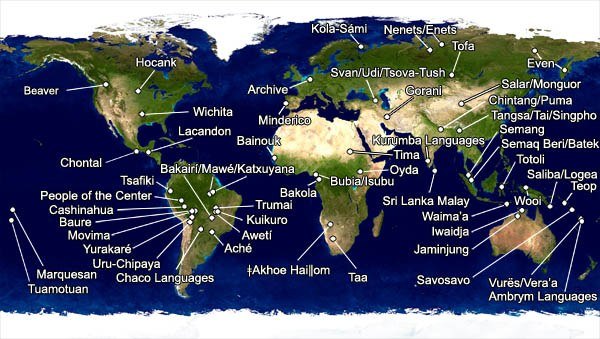
\includegraphics[width=\textwidth]{.\imgpath/Bouda-img7.jpg}
\caption{The DOBES documentation projects \url{http://www.mpi.nl/dobes}}
\end{figure}


Language documentation is a multi-purpose enterprise, but one important purpose of DOBES corpora is to serve as data bases for grammatical descriptions of these languages. Since these corpora have a different structure and different properties than the large monolingual corpora that are available for English, German and other major European languages they allow for and require different corpus linguistic methods. Or, to put it the other way round, corpus linguistic methods have to be adapted to the specific properties of DOBES corpora.

One of the great advantages of DOBES corpora over these traditional corpora is that they are always bilingual with an idiomatic translation in one of the main European languages, and in addition, that they often include a morpheme-by-morpheme glossing. This means that DOBES corpora contain much more additional information in form of these types of annotations than traditional corpora. The large monolingual corpora mostly consist of plain text only. It is the overall goal of this article to show how corpora such as DOBES corpora can be exploited by corpus linguistic means in order to extract the kind of data that are necessary for grammatical descriptions. 

What kind of data is necessary for a grammatical description can be deduced from the principles and requirements of grammaticography. One important distinction that is maintained in grammaticography is the one between a semasiological and an onomasiological approach to grammar. 

The semasiological approach takes the formal expressions of a language as starting point and tries to find out what they mean in different contexts. This approach resembles the analytic tasks hearers have to fulfill in interpreting speakers' utterances. They have to start from the uttered expression and have to assign a meaning to them which is appropriate in the given shared context of the utterance. 

The onomasiological approach, on the other hand, takes the meaning/ function as starting point and tries to find out which forms in a language may be used to express them. This approach resembles the generative task the speaker has to fulfill in order to form an utterance. The speaker has a concept of what he/she wants to communicate to the hearer and his/her task is to find the appropriate expression in a given shared context that fulfills the intended meaning best.

These different but complementary approaches to grammar have also an impact on the data searching methods to be applied to the corpus. The semasiological approach dominates in traditional computational treatments of monolingual text corpora. Specific lexical or grammatical forms in the target language are searched for in digital corpora. The goal is to collect all different contexts in which these forms appear in order to find out the conventional meanings of these forms and their variation in different contexts. 

The onomasiological approach, on the other hand, requires a semantic annotation such that all forms and constructions that express a certain semantic notion -- for instance possession -- are annotated in a way that the search for the annotation ``possession'' gives all different expressions of this notion. A semantic annotation is -- of course - the rare exception in digital corpora, since they have to be added manually, which is a quite time-consuming process. 

It is one of the main goals of this paper to show that the particular strength of DOBES corpora is that they can be exploited much more systematically than traditional monolingual corpora. They allow for searches that provide the necessary data for both the semasiological and the onomasiological approach in direct and indirect ways. The second goal of this paper is to present a linguistic database and concordancing software -- the Poio Analyzer - that allows easily - i.e. in a user friendly manner -- to conduct the text searches that are necessary to extract the kinds of data from a DOBES corpus that are required for the two different analytical approaches to grammar just mentioned. 

The structure of the paper is as follows. The main properties of DOBES corpora and their implications for the various search types will be dealt with in Section\ \ref{bouda:sec:structureandproperties}. Section\ \ref{bouda:sec:typologyofsearches} presents a general typology of possible search types within DOBES corpora. These search types are -- in principle -- independent of the two approaches to grammar and the types of data they require. It will be demonstrated that these kinds of searches exceed the possibilities that monolingual corpora allow for. In Section\ \ref{bouda:sec:structuralgrammar}, it will be exemplified how these search types can be utilized to gain data that are relevant for a semasiological description. In Section\ \ref{bouda:sec:functionalgrammar}  in turn, it will be exemplified how data may be extracted from a DOBES corpus - using these search types - that are relevant for the onomasiological description. In Section\ \ref{bouda:sec:softwarebasesearch}  and Section\ \ref{bouda:sec:poioanalyzer}, the functionality and the shortcomings of Elan with regard to concordances will be evaluated and the prototype of a linguistic database and concordancing software -- the Poio Analyzer - will be introduced that is designed specifically for the needs of a descriptive linguist.

\section{The structure and properties of DOBES corpora}%\label{bkm:Ref283033309}
\label{bouda:sec:structureandproperties}
The typical structure of an annotated text of a DOBES corpus can be seen in Figure  \ref{bouda:fig:corpussentence}. An annotated text consists minimally: a) of a text tier (abbreviated \textit{tx} in Figure \ref{bouda:fig:corpussentence}) containing the transcribed text of the audio and video recording, and b) a free idiomatic translation tier (abbreviated \textit{ft} in Figure  \ref{bouda:fig:corpussentence}). Many DOBES corpora have, in addition, a morpheme-by-morpheme glossing such that there is c) a tier with a morpheme segmentation (abbreviated \textit{mo} in Figure  \ref{bouda:fig:corpussentence}) and d) a tier with lexical and grammatical glosses corresponding to the segmented morphemes in the \textit{mo} tier (abbreviated \textit{gl} in Figure  \ref{bouda:fig:corpussentence}).

\begin{figure}
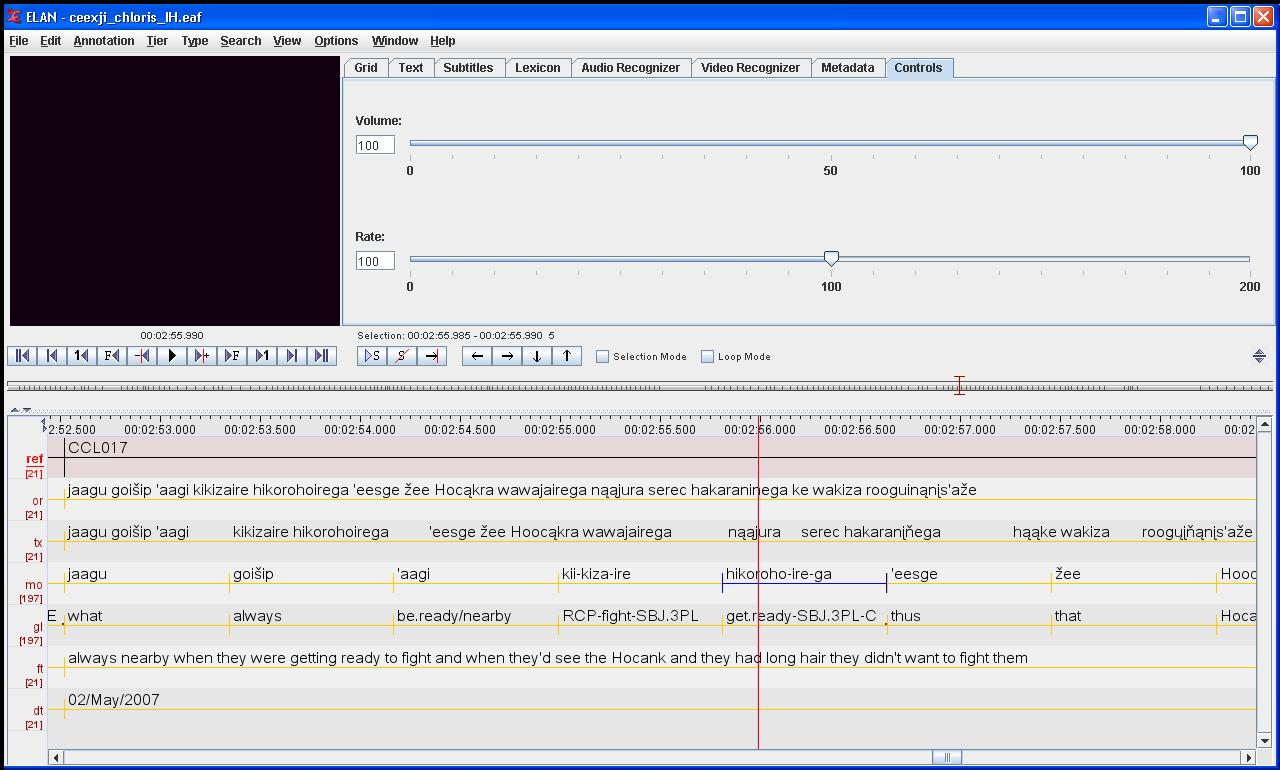
\includegraphics[width=\textwidth]{.\imgpath/Bouda-img8.jpg}
\caption{Screen shot of an annotated Hoc{\A}k (Siouan) sentence in Elan}
\label{bouda:fig:corpussentence}
\end{figure}



The tx tier contains the usually time-aligned transcription of the audio/video recording. These transcriptions are usually not based on the IPA, but on an already existing conventional orthography, or on a practical orthography developed by the documentation team. Associated with the tx tier there is a ft tier which contains the free or idiomatic translation of the target language text. The language used for the free translation is usually one of the major European languages often the one that replaces the endangered language in the community. In the example in Figure  \ref{bouda:fig:corpussentence}, this is English. Many documentation teams enriched the transcription in the tx tier and its translation in the ft tier with a second type of translation called lexical and grammatical morpheme-by-morpheme glossing. For this, a morpheme segmentation in the mo tier is matched with a gl tier that contains the lexical or grammatical glosses; cf. Figure  \ref{bouda:fig:corpussentence}.

It has to be kept in mind that these four essential parts of an annotated text involve previous and preliminary decisions on the side of the linguist that may turn out to be wrong later on in the process of the advancing documentation.

\ea
 With regard to the text tier (tx):
 \begin{enumerate}
 \item The practical orthography developed by the documentation team may be based on a wrong phonological analysis;

 \item The segmentation of the text in sentence/ utterance units may turn out to be wrong later on;

 \item The segmentation of the text into words may turn out to be wrong later on;

 \end{enumerate}
\z

\ea
 With regard to the translation tier (ft):
 \begin{enumerate}
 \item The free translation into the European language may be semantically incomplete (i.e. certain forms of the target language are not translated and are left to inference) or may contain semantic elements that are only implied in the text of the target language but are obligatory in the mediating language; 
 \end{enumerate}
\z

\ea
 With regard to the morpheme and gloss tiers (mo/gl):
 \begin{enumerate}
 \item The identification of the grammatical and lexical morphemes and their status may turn out to be wrong later on;
 \item Or, the assignment of grammatical function/ lexical meaning to a lexical or grammatical form may be wrong or incomplete;
 \end{enumerate}
\z

The main goal of the documentation of an endangered language is not the grammatical analysis of the language \textit{per se}, but the collection and processing of a representative corpus of texts in a way that a non-speaker can access it. It is hence obvious that the list of grammatical forms and lexical items has to be preliminary in the documentation process itself. However, even if there are mistakes in the transcriptions, in the translations, and in the morpheme-by-morpheme glossing, all three elements of the annotation represent an invaluable source of additional information that can be exploited in corpus linguistic searches. DOBES corpora are parallel corpora relating a morpheme-by-morpheme translation as well as a free translation to the text of the target language. This kind of additional information presupposes a preliminary phonological analysis (with regard to the transcription) as well as a preliminary grammatical analysis (with regard to the glossing). It will be shown in a moment that digital corpora of this DOBES type allow types of searches that are interesting for descriptive purposes and that go beyond the possibilities of traditional monolingual corpora. These additional search possibilities will be systematically explored in the following section.

\section{A typology of corpus linguistic searches in DOBES corpora}
% \label{bkm:Ref296525673}\label{bkm:Ref283033343}
\label{bouda:sec:typologyofsearches}

From a technical point of view the search types a descriptive linguist would like to apply to a DOBES corpus are independent of the distinction between the two basic approaches to grammar mentioned above. The most important search types are summarized in Search for a single lexical or grammatical form F1 or a single construction C1 consisting of more than one element in a single tier x1 within a linguistic context defined by the level of syntagmatic complexity/ grammatical level: and Search for the co-occurrence of two or more lexical or grammatical forms F1 and F2, or of construction C1 and C2 in one specific tier x1 or across different tiers x1-n within a linguistic context defined by the level of syntagmatic complexity/ grammatical level:.

\ea
 \begin{itemize}
\item \label{bkm:Ref283731549}Search for a single lexical or grammatical form F\tief{1} or a single construction C\tief{1} consisting of more than one element in a single tier x\tief{1} within a linguistic context defined by the level of syntagmatic complexity/ grammatical level:

 \begin{enumerate}
 \item[a)] tier x\tief{1} [...F\tief{1}...]\tief{word} [...C\tief{1}{}-C\tief{1}...]\tief{word}

 \item[b)] tier x\tief{1} [...F\tief{1}...]\tief{phrase} [...C\tief{1}{}-C\tief{1}...]\tief{phrase}

 \item[c)] tier x\tief{1} [...F\tief{1}...]\tief{clause/sentence} [...C\tief{1}{}-C\tief{1}...]\tief{clause/sentence}

 \end{enumerate}
\end{itemize}
Comments:

\begin{itemize}
\item Forms or constructions may be searched within all kinds of tiers, i.e. tier x\tief{1} = \{tx, mo, gl, ft, ...\}

\item F\tief{1} stands for a string of characters that does not exceed the word boundary, e.g. a submorpheme, a morpheme, a word, a lexical or grammatical gloss, a word of the language of translation, etc.\}

\item C\tief{1} stands for any discontinuous chain of linguistic units with a conventionalized meaning within a certain level of syntagmatic complexity, for instance circumfixes on the word level, or analytic constructions such as the \textit{will} + Verb\tief{\textsc{in}F} future construction in English;
\end{itemize}

The Search results should be presented in an interlinear version. It should be possible to store the search results/ hits as a separate data set which may be the basis for another search. It should be possible that the context size of the concordances can be determined with respect to the different levels of syntagmatic complexity (see below Table \ref{bouda:tab:gramunits}).
\z

% \ea 
Search for the co-occurrence of two or more lexical or grammatical forms F\tief{1} and F\tief{2}, or of construction C\tief{1} and C\tief{2} in one specific tier x\tief{1} or across different tiers x\tief{1-n} within a linguistic context defined by the level of syntagmatic complexity/ grammatical level:
 \begin{enumerate}
 \item[a)] tier x\tief{1} [...F\tief{1}/C\tief{1}{}-C\tief{1}...F\tief{2}/C\tief{2}{}-C\tief{2}...]\tief{word/ phrase/ clause/ sentence}

 Between the linguistic items (i.e. forms/ constructions) F\tief{1-2}/C\tief{1-2} which are searched for in this search type -- on a single tier x\tief{1} - a logical operation can be defined such F\tief{1} \{AND, OR, AND NOT etc.\} F\tief{2}, or F\tief{1} \{AND, OR, AND NOT etc.\} C\tief{1}{}-C\tief{1}, and so forth.

 \item[b)] tier x\tief{1} [...F\tief{1}/C\tief{1}{}-C\tief{1}...]\tief{ word/ phrase/ clause/ sentence} and tier x\tief{2} [...F\tief{2}/C\tief{2}{}-C\tief{2}...]\tief{ word/ phrase/ clause/ sentence}

 Between the linguistic items F\tief{1 }in tier x\tief{1} and F\tief{2} in tier x\tief{2} or C\tief{1} in tier x\tief{1} and C\tief{2} in tier x\tief{2}, and so forth, which are searched for in this search type, a logical operation can be defined such that F\tief{1} in tier \tief{1} \{AND, OR, AND NOT etc.\} F\tief{2} in tier x\tief{2}, or C\tief{1}{}-C\tief{1} in tier x\tief{1} \{AND, OR, AND NOT etc.\} C\tief{2}{}-C\tief{2} in tier x\tief{2}, and so forth.

 \end{enumerate}
% \z 


The principle types of corpus linguistic searches summarized in an abstract form in Search for a single lexical or grammatical form F1 or a single construction C1 consisting of more than one element in a single tier x1 within a linguistic context defined by the level of syntagmatic complexity/ grammatical level:{}-Search for the co-occurrence of two or more lexical or grammatical forms F1 and F2, or of construction C1 and C2 in one specific tier x1 or across different tiers x1-n within a linguistic context defined by the level of syntagmatic complexity/ grammatical level: will be applied to specific data needs of the two complementary approaches to grammar in the subsequent sections (cf. Sections\ \ref{bouda:sec:structuralgrammar} and \ref{bouda:sec:functionalgrammar}). Different questions in a semasiological approach and an onomasiological approach will be posed and it will be show how these different questions could be translated into different kinds of searches. The illustrating examples come from the Hoc{\A}k corpus \citep{HartmannEtAl2009hocank}, a DOBES corpus compiled within the DOBES project ``Documentation of the Hoc{\A}k Language'' some years ago.\footnote{Cf. 
 the website of the DOBES project ``Documentation of the Hoc{\A}k Language'' \url{http://www2.uni-erfurt.de/sprachwissenschaft/Vgl_SW/Hocank/index_frames.html} 
} 

\section{Structural grammar -- the semasiological approach}
\label{bkm:Ref283033396}
\label{bouda:sec:structuralgrammar}

The goal of a structural grammar is to identify the lexical and grammatical units (including grammatical constructions), and to find out the syntagmatic possibilities of the combinations of these units on all syntagmatic levels of complexity. There are at least four such levels of complexity: the word, the phrase, the clause (or simple sentence), and the complex sentence, cf. Table  \ref{bouda:tab:gramunits}.

\begin{table}
\begin{tabular}{p{6cm}p{6cm}}
 \textbf{grammatical units} & \textbf{levels of syntagmatic complexity}\\\hline
 submorpheme & word\\\hline
 lexical and grammatical morphemes (stems and affixes) and their combinatory possibilities & word\\\hline
 lexical and grammatical words and their combinatory possibilities & phrase\\\hline
 phrase & clause\\\hline 
 clause & (complex) sentence\\\hline
 sentence & text/ discourse\\
\end{tabular}
\caption{Grammatical units and the levels of complexity}
\label{bouda:tab:gramunits}
\end{table} 

On the word level, the descriptive linguist has to identify all lexical and grammatical morphemes of a language, their respective paradigms, and all rules of syntagmatic combinations of bound morphemes with lexical morphemes. This task implies among other things that word forms -- the primary empirical basis of this task -- have to be compared in order to find stem and affixes. This task is easier to solve if there is a preliminary analysis available in form of a morpheme-by-morpheme glossing. 

On the phrase level, the descriptive linguist has to identify all lexical and grammatical words and their possible combinations in phrases. This task is easier to solve if there is a parts-of-speech annotation which, unfortunately, is lacking systematically in DOBES corpora. 

And last but not least, on the level of the clause and complex sentence, the descriptive linguist has to determine all phrase types and their possible combinations in clauses and complex sentences. This task would be easier to solve, if there were a phrase structure annotation which is lacking in DOBES corpora as well. 

One may say that the better or richer the annotations the easier are the problems of a structural grammar to solve. Whether a text corpus comprises a morpheme-by-morpheme glossing or not makes a big difference with regard to the formulation of searches in the text corpus and the exactness and relevance of the hits one gets out of these searches. The subsequent sections illustrate some corpus linguistic methods that can be applied to DOBES corpora in order to gain data that are relevant for a structural grammar and the semasiological approach to grammar. These illustrations remain on the word level. On the higher levels of syntagmatic complexity the lack of a parts of speech and phrase structure annotation in DOBES corpora complicates the application of corpus linguistic methods. The descriptive linguist has to find indirect searches in order to identify the syntactic units a language ahs above the word level.

\subsection{Identification of lexical units}\label{bouda:sec:identificationoflexicaluntis}

Words - word forms to be more precise - can be identified in the transcription line (tx tier) by blanks at the left and the right edge. However, problematic cases arise for instance with clitics and compounds. The transcription team necessarily decided at some point in the documentation that a certain form is a clitic, or not, by using blanks. The problem is that this decision may be wrong or inconsistent throughout the corpus for various reasons (e.g. progress or changes in grammatical analysis during the transcription process, inconsistent analysis on the basis of different criteria, native speakers changing intuition etc.). Furthermore, the decision whether a combination of nouns is a coordination of phrases or a nominal compound may be difficult to draw, if there are no morphological markers that indicate this kind of relation; therefore the transcription may be inconsistent with regard to this question too. 

The identification of lexical units requires that all forms of a lexeme (including stem allomorphs) and the lexeme itself are identified together with its conventional meaning (polysemy included). Homophonous forms should be found also. There are two possibilities with regard to a DOBES corpus, either the corpus has a morpheme-by-morpheme segmentation/glossing (cf. next subsection Section\ \ref{bouda:sec:identificationoflexicaluntiswomorpheme}), or not (cf. Section\ \ref{bouda:sec:morphmebymorphemeglossing}). 

\subsubsection{Identification of lexical units: without morpheme segmentation and glossing in the corpus}
\label{bouda:sec:identificationoflexicaluntiswomorpheme}

There are three possible strategies in order to identify lexical stems: 

a) One may export all words of the target language (defined by blanks in the text corpus) and list them alphabetically. Words of the same form are simply counted; the stems of inflected or derived word forms can be found by comparison: the larger stem parts of the words are identical or at least similar. See Table  \ref{bouda:tab:hocankwordlist} for an example of this procedure from the Hoc{\A}k corpus. 

\begin{table} 
\begin{multicols}{3}
\textbf{x{\U}n{\U}}{\II}g 2

\textbf{x{\U}n{\U}}{\II}ga 1

\textbf{x{\U}n{\U}}{\II}gn{\A} 1

\textbf{x{\U}n{\k{\'u}}}{\II}gn{\A}{\A}gre 1

\textbf{x{\U}n{\U}}{\II}gn{\A}{\A}gre 2

\textbf{x{\U}n{\U}}{\II}gra 1

\textbf{x{\U}n{\U}}{\II}g\v{s}{\A}n{\A} 1

\textbf{x{\U}n{\U}}ik 1

\textbf{x{\U}n{\k{\'u}}}{\II}k 1

\textbf{x{\U}n{\U}}{\II}k 3

\textbf{X{\U}n{\k{\'u}}}{\II}ka 1

\textbf{x{\U}n{\U}}{\II}kra 2

\textbf{x{\U}{n{\k{\'u}}}{\II}kregi 1}

\textbf{x{\U}n{\U}}n{\A} 1

\textbf{x{\U}n{\k{\'u}}}n{\A}{\A}k\v{s}{\A}n{\A} 1

\textbf{x{\U}n{\U}}n{\II}{\II}sge 1

\textbf{x{\U}n{\U}}n\k{\'{i}}k 1

\textbf{xun{\U}}xj\k{\'{i}} 1

\textbf{x{\U}n{\U}}xj{\II} 1

\textbf{x{\U}n{\k{\'u}}}xj{\II}n{\II}k 1

{Xurucre 2}

{xusgajan{\A} 1}

{xuu 3}

{x{\U}{\U}n{\U} 3}

{x{\U}{\U}n{\U}{\II}g 1}

{x{\U}{\U}n{\U}{\II}gi\v{z}{\A} 1}

{x{\U}{\U}n{\U}{\II}gn{\A}{\A}ka 2}

{x{\U}{\U}n{\k{\'u}}{\II}gn{\A}ka 1}

{x{\U}{\U}n{\U}{\II}gra 1}

{x{\U}{\U}n{\U}{\II}k 3}

{x{\U}{\U}n{\U}{\II}kra 1}

{x{\U}{\U}n{\U}n\k{\v{a}} 5}

{x{\U}{\U}n{\U}n{\A}ka 1}

{X{\U}{\U}n{\U}n{\II}kga 1}

{x{\U}{\U}n{\k{\'u}}n{\II}kjeega 1}

{x{\U}{\U}n{\U}n{\II}kra 1}

{x{\U}{\U}n{\U}xj\k{\'{i}} 1}

{x{\U}{\U}nuxj{\II}gra\v{s}ge 1}

{x{\k{\'u}}{\U}n{\U}xj{\II}n{\II}kra 1}

{x{\U}{\U}n{\U}\v{z}e 1} 
\end{multicols} 
\caption{Extract from the word list of the entire Hoc{\A}k corpus: \textit{x{\U}n{\U}}  `small, little'}
\label{bouda:tab:hocankwordlist}
\end{table}


Table \ref{bouda:tab:hocankwordlist} contains a segment of all word forms of the Hoc{\A}k corpus alphabetically sorted. This wordlist was compiled and exported with Elan. The segment in Table \ref{bouda:tab:hocankwordlist} contains all word forms that resemble the lexeme \transcr{x{\U}n{\U}}{small, little} in the corpus. As can be seen in this list, there are derived forms of \transcr{x{\U}n{\U}}{small, little} with different suffixes, and there are compounds of \transcr{x{\U}n{\U}}{small, little} with other lexemes. In addition, it is obvious that there are inconsistent spellings of \transcr{x{\U}n{\U}}{small, little}, the forms in bold with short vowels, the forms in the last two columns with a long stem vowel. Nevertheless, this method allows identifying stems by means of comparison of the similar word forms and, in addition, it is possible to some degree to identify the allomorphs of the lexical morpheme. A problem arises with prefixed word forms. They appear in another segment of the alphabetical list of words, but see Figure \ref{bouda:fig:concordances} below. The list in Table \ref{bouda:tab:hocankwordlist} exhibits also a minor technical problem with Elan, the annotation software with which the word list was generated. Elan ignores the nasal /\textit{{\U}}/ vs non-nasal /u/ in the sort order, so that different words appear in the middle of the list (e.g. \transcr{xuu}{leg}), it also ignores stressed vowels which is, however, helpful in this case.

b) The second strategy may be to search for strings which are hypothetically part of the word stems in the object language (using regular expressions, if necessary); for instance, if you search for \textit{x{\U}n{\U}} 'small' in the tx tier of the corpus, you'll get 37 hits, among them also forms with prefixes as can be seen in the concordances in Figure \ref{bouda:fig:concordances} below. The advantage of this strategy is that you get prefixed and suffixes as well as compounded forms of the hypothetical stem. The disadvantage, however, is that spelling alternations and stem allomorphy is ignored.
% 
% \begin{table} 
% \begin{tabular}{p{5cm}lp{5cm}}
% ``{s'iireja} &
% {h\k{i{x{\U}n{\U}}{\II}gregi}} &
% {hi'{\U}n{\II} haara taan{\II}\v{z}u n{\A}{\A} 'eeja ruus\v{s}{\U}n{\U}regi hagijite\v{s}{\U}n{\U}}''\\\hline
%  &
% {``h\k{i{x{\U}n{\U}}\v{n}eegi}} &
% {heg{\U} haahe teegi \v{z}oo\v{z}ocra roigixrawii\v{s}un{\U}.}''\\\hline
%  &
% {``h\k{i{x{\U}n{\U}}{\II}gregi\v{s}ge}} &
% {hicooke haara\v{s}ge wa\v{z}{\A}n{\A} rooh{\A}xj{\II} h{\U}{\U}kirakra waak{\II}k{\U}n{\U}n{\II} waa'{\U}n{\A}k\v{s}{\A}n{\A}}''\\\hline
%  {``h{\A}h{\A}; x'ookera} &
% \textbf{{x{\U}n{\U}}{\II}gn{\A}{\A}gre} &
% {jaasge wagigires'agi tee tee hi\v{z}{\A} hi\v{z}{\A} wagan{\A}{\A}gre}''\\\hline
%  {``h{\A}h{\A}, jaasge} &
% {h\k{i{x{\U}n{\U}}{\II}gjeegi\v{s}{\A}n{\A}}} &
% {hahi woto\v{g}ocn{\II}sge\v{s}{\U}n{\U}}''\\\hline
%  {``horu\v{s}j{\A} hi\v{z}{\A} heg{\U} tee heg{\U} tee heg{\U} hagorei\v{z}{\A} Heen{\A}ga tee hi\v{z}{\A} Heen{\A}} &
% \textbf{{x{\U}n{\U}}n{\A}} &
% {Emmanuelga horujisra (hi??)\v{z}{\A} hagorei\v{z}{\A} heg{\U}}''\\\hline
%  {``hija 'an{\A}ga heg{\U}...} &
% {wa\v{z}{\A}su}\textbf{{x{\U}n{\U}}{\II}g} &
% {n{\II}{\II}sge jagu\v{s}ge wigairera?}''\\\hline
%  {``heg{\U}} &
% \textbf{{x{\U}n{\U}}{\II}g\v{s}{\A}n{\A}''} &
% \\\hline
%  {``gota\v{s}ge wa\v{z}{\A} hee wigan{\A}k 'eegi ceerap} &
% {h{\II}x{\U}n{\U}wiregi} &
% {ceerap wiagawi\v{s}{\U}n{\U}}''\\\hline
%  {``N{\II}kuse} &
% {(Ho)}\textbf{{x{\U}n{\U}}\v{n}{\A}} &
% {\v{z}e'e\v{s}ge that's the Wisconsin River \v{z}ee ho'{\U}{\II}\v{n}ekjanen{\A} N{\II}oxawan{\II}ra\v{s}ge ho'{\U} hikiware hikiwarairekjanera \v{z}ee 'eeja '{\U}{\II}\v{n}ekjanen{\A}}''\\\hline
%  {``P{\II}hi wes\k{\'{i}}w{\II}-gaj{\A} tew\'oiraki n{\II}\v{s}\'an{\A}k} &
% \textbf{{x{\U}n{\k{\'u}}}xj{\II}n{\II}k} &
% {.-h\'i\v{z}{\A}; hat'{\A}pji-\'an{\A}ga wa'{\U}j\'e\v{z}e.''}
% 
% \end{tabular}
% \caption{Selected concordances of a search of \textit{x{\U}n{\U}} `small'}
% \label{bouda:tab:concordances}
% \end{table} 

\begin{figure}
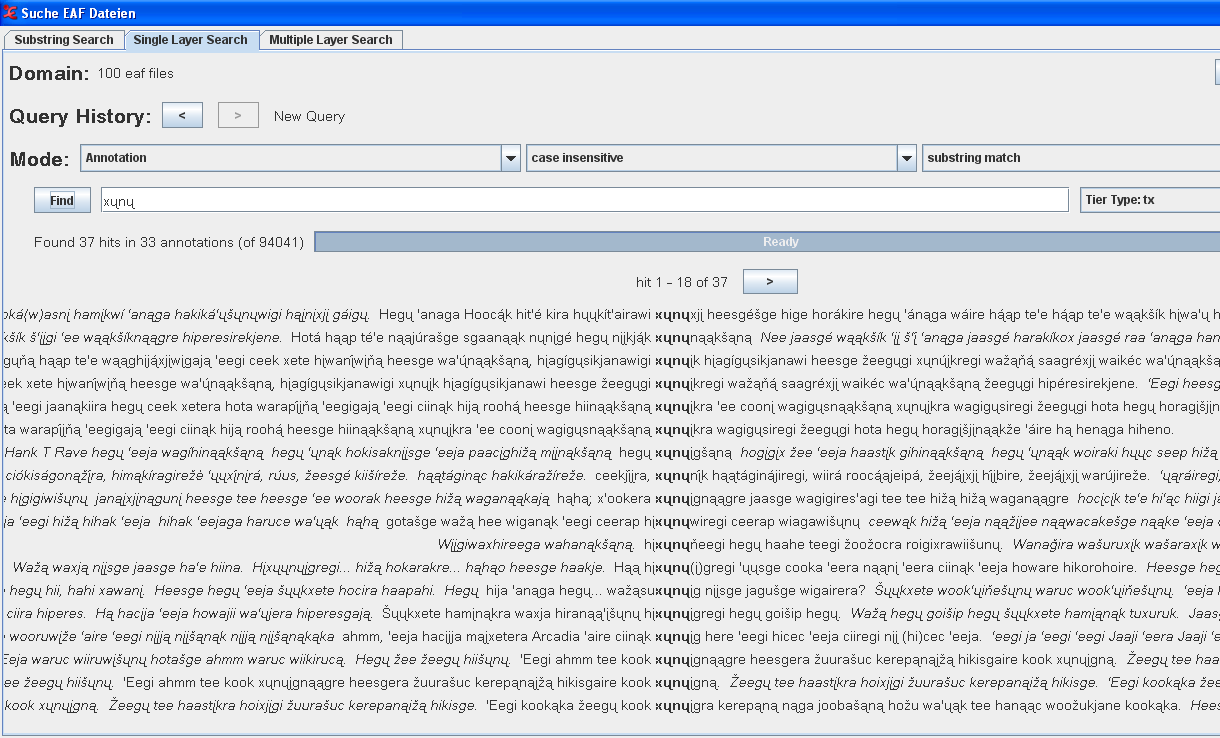
\includegraphics[width=\textwidth]{.\imgpath/BoudaKonkordanz.png}
\caption{Selected concordances of a search of \textit{x{\U}n{\U}} `small'}
\label{bouda:fig:concordances}
\end{figure}

c) The third strategy starts from the translation tier. One may search for a lexical item in the free translation ft tier assuming that there is a lexical match in the object language. For instance, if you search for \textit{small/little} in the ft tier, you indeed get lexical matches in the target language, cf. \xref{bouda:ex:ED3024}, or you get forms with a diminutive marker (glossed DIM) as can be seen in \xref{bouda:ex:CTD003}. 

\newpage
\let\eachwordthree=\rm
\ea\label{bouda:ex:ED3024}
ref ED3024
\glll 
tx cii x{\U}{\U}n{\U}{\II}k hi\v{z}{\A} '{\U}{\U}    \\
mo cii x{\U}{\U}n{\U}-{\II}k hi\v{z}{\A} '{\U}{\U}     \\
gl house be.small(\textsc{obj}.\textsc{3sg})-\textsc{dim} one do/make(\textsc{sbj}.\textsc{3sg})      \\\

\glll 
tx jaagu n{\II}{\II} hicec 'eeja \\
mo jaagu n{\II}{\II} hicec \\
gl  what water near\\

ft he made a small house by the river\\
dt 25/Oct/2004\\
\z
 
\ea\label{bouda:ex:CTD003}
ref CTD003
\glll 
tx \v{z}ee ceek hon{\U}w{\A}k 'eeja tee hoc{\II}c{\II}gi\v{z}{\A}, n{\II}{\II}kj{\A}k n{\A}{\A}gre \\
mo \v{z}ee ceek ho-n{\U}w{\A}k 'eeja tee hoc{\II}c{\II}-{\II}g-i\v{z}{\A} n{\II}{\II}kj{\A}k n{\A}{\A}gre\\
gl that first/new \textsc{appl}.\textsc{iness}-run there this \textbf{boy-\textsc{dim}-one} child these\\
ft from the start, \textbf{a little boy}, these children...ahm... \\
dt 11/May/2006\\
\z

In \xref{bouda:ex:ED3024}, the result of the search is the expected property word \textit{x{\U}{\U}n{\U}-{\II}k '}small-DIM', however, with the diminutive marker \textit{--(n){\II}k}; in \xref{bouda:ex:CTD003}, there is no lexical equivalent of the search item 'small', instead one gets a noun with a diminutive marker only. This strategy has the advantage to provide an overview of the forms in the target language that correspond a specific form of the language of translation. It is hence a search type that rather belongs to the onomasiological approach. In addition, it allows the identification of the allomorphs of a morpheme. Another advantage is that this strategy allows the finding of lexical paradigms and stem suppletivism. The disadvantage is that this strategy ignores the polysemy (manifest as variation in the translation) of a form.

\subsubsection{With morpheme-by-morpheme glossing in the corpus}
\label{bouda:sec:morphmebymorphemeglossing}
The identification of lexical stems is of course much easier, if there are morpheme breaks and a glossing of the lexical and grammatical morphemes. The morpheme-by-morpheme interlinear glossing presupposes an analysis of lexical and grammatical forms. The mo tier contains the underlying or standardized form of the grammatical and lexical morpheme, and the gl tier attributes the standard glossing (\textit{Grundbedeutung}) of the morpheme. Searches of the lexical item on the mo tier allow finding the allomorphs of a lexical morpheme by comparing the hits with the corresponding form on the tx tier. For instance, in the Hoc{\A}k corpus, there are quite a few variously abbreviated forms of \textit{an{\A}ga} 'and' such as \textit{-n{\A}ga} in the tx tier which could not be found otherwise. These forms are allomorphs of \textit{an{\A}ga}.

\subsection{Identification of grammatical units}

The Identification of grammatical units requires the establishment of the morpheme-allomorph pairings and its grammatical meanings or functions. With respect to corpus linguistic searches in DOBES corpora, there are two possibilities: either the corpus has a morpheme-by-morpheme segmentation/glossing, or not. 

\subsubsection{Identification of grammatical units: without morpheme segmentation and glossing in the corpus}
The methods to be applied here are quite similar to the ones applied for the identification of lexical units, see above Section\ \ref{bouda:sec:identificationoflexicaluntis}. The first strategy is to export all words of the target language (defined by blanks in the text corpus) and list them alphabetically. The inflected and derived word forms will show up in the list if the stems remain formally constant and have no prefixes. One has to look for systematic variations with regard to form-meaning pairings in the tx line and the ft line. If there are systematic form-meaning variations with respect to some affix-like form or with respect to some potential grammatical words, one can proceed with searching these forms in the text tx tier. For instance, in Hoc{\A}k, progressive aspect is systematically expressed by means of certain verb-auxiliary analytical constructions. Once the construction is discovered, one may search these constructions systematically on the tx tier.

Another strategy could start with prototypical nouns and verb, since grammatical variation can be expected to occur primarily with words of the open classes. These prototypical nouns and verbs have to be looked for in the translation ft tier. Under the assumption that for instance inflected verbs in the translation ft tier correspond to inflected verbs in the text tx tier, one may start with searches for prototypical verbs and nouns in the ft tier. This strategy can be applied also to grammatical meanings: grammatical meanings such as personal pronouns ('I', 'you', etc.), progressive aspects (e.g. 'V-\textit{ing}'), and so forth can be searched for in the translation ft tier. The results can be compared with what corresponds to it in the tx line of the object language. The problem with this kind of search is that one will not find complete paradigms in the text corpus. Elicitation of forms with a native speaker is much more promising here as a strategy.

The latter strategy can be exemplified with an example from the Hoc{\A}k corpus. If one want to find out, if progressive aspect (PROG) is marked grammatically in Hoc{\A}k, one may search for \textit{V-ing} constructions in the translation ft tier. Of course, the range of hits one gets is much wider than just the clear progressive uses of this form, since the \textit{--ing} form in English is not restricted to progressive aspect. So, one has to select from the results of this search the cases which seem to be good cases of a progressive meaning in English and may compare this with the forms in the text tx tier.

A variation of this kind of search is to choose a specific probably frequent verb and search for its progressive construction in the translation tier. For example, a search for ``was looking'' receives 6 hits in the Hoc{\A}k corpus with quite interesting results. First of all, one gets the standard analytic construction in Hoc{\A}k for the expression of progressive aspect (cf. the text in bold in the second line of example \xref{bouda:ex:TWI026} corresponding to the English meaning 'listening to them'); it is one possible verb auxiliary construction for progressive aspect; but one gets also an alternative expressions such as the reduplication (cf. first line in example \xref{bouda:ex:TWI026} which corresponds to 'was looking'), and more astonishing, a construction with the habitual marker (glossed \textsc{hab}) on the verb, cf. \xref{bouda:ex:HOR029}. 


\ea\label{bouda:ex:TWI026}
ref TWI026
\glll 
tx Heg{\U} heg{\U} han\'{\A}{\A}c horo\v{g}\'o\v{g}oc heg{\U}          \\
mo heg{\U} heg{\U} han{\A}{\A}c     horo$<$\v{g}o$>$\v{g}oc heg{\U}         \\
gl that.way that.way all \textbf{$<$\textsc{rdp}:\textsc{iter}$>$look.at(\textsc{sbj}.\textsc{3sg})} that.way     \\
\glll
tx wan\'{\A}xg{\U} wa'{\U}{\A}k\v{s}{\A}n{\A} heg{\U} {} \\ 
mo wa-n{\A}{\A}xg{\U} wa'{\U}-'{\A}k-\v{s}{\A}n{\A} heg{\U} \\
gl \textbf{\textsc{obj}.\textsc{3pl}-hear(\textsc{sbj}.\textsc{3sg})} \textbf{do/be-\textsc{pos}.\textsc{hor}-\textsc{decl}} that.way\\

ft It was looking all around and listening to them.\\
dt 21/Sep/2006\\
\z
 
\ea\label{bouda:ex:HOR029}
ref HOR029
\glll 
tx Hoto\v{g}ocnaga heg{\U} \v{s}{\II}{\II}cra\v{s}ge n{\A}{\A}sura...     hoip{\II}n{\II} \\
mo hoto\v{g}oc-n{\A}ga heg{\U} \v{s}{\II}{\II}c-ra-\v{s}ge n{\A}{\A}su-ra hoip{\II}n{\II}   \\
gl look.at{\textbackslash}\textsc{1e.a}-and that.way rear-\textsc{def}-also head-\textsc{def}        spin                \\
\glll
tx haakirin{\A}k heg{\U}        hakjopahi\v{s}ge              \\
mo ha$<$ha$>$kirin{\A}k heg{\U} hakja-ho-hapahi-\v{s}ge         \\
gl $<$1\textsc{e.a}$>$land.on that.way   back-\textsc{appl}.\textsc{iness}-go.toward-also    \\
\glll
tx ham{\II}{\A}n{\A}kn{\A}ga\v{s}ge, c{\A}{\A}geja g{\U}{\A}gaira horo\v{g}ocn{\II}{\II}sge\v{s}{\U}n{\U}.\\
mo ham{\II}$<$ha$>$n{\A}k-n{\A}ga-\v{s}ge c{\A}{\A}k-'eeja g{\U}{\A}gaira horo\v{g}oc-n{\II}{\II}sge-\v{s}{\U}n{\U} \\
gl  $<$1\textsc{e.a}$>$sit.on-and-also outside-there sometimes look.at-\textsc{vague}-\textsc{hab}\\

ft I got on it and spun around on it \textbf{glancing} outside once and a while, while I \textbf{was looking} over the back end.\\
dt 22/Sep/2006\\
\z



Especially the latter result is due to the polysemy of the English progressive aspect on \textit{--ing} which obviously can be used to express habitual meanings too. The latter type of search equally belongs to the onomasiological approach to grammar.

\subsubsection{With a morpheme-by-morpheme segmentation and glossing in the corpus}
If grammatical morphemes are already glossed, it is of course easy to find all its allomorphs and all its meanings. Just look for the grammatical gloss on the gloss tier. For instance, if one looks for the Hoc{\A}k future tense marker glossed \textsc{fut} one finds at least five different forms (allomorphs) for this marker --\textit{kjene} '\textsc{fut}', cf. Table \ref{bouda:tab:future}. 

\begin{table}
\begin{tabular}{lll}
 \textbf{allomorphs} &
 \textbf{grammatical meanings/functions} &
 \textbf{gloss}\\\hline
\parbox{2cm}{
  \textit{-kje }\\
  \textit{-kjane}\\
  \textit{-kjene}\\
  \textit{-kj{\A}n{\A}he}\\
  \textit{-kjenehe}
} 
&
future intentional, irrealis, desiderative, obligation &
\textsc{fut}\\
\end{tabular}
\caption{Allomorphs of the future tense marker \textit{--kjene} \textsc{fut} in the Hoc{\A}k corpus}
\label{bouda:tab:future}
\end{table}

The results of this search show that there is some allomorphy associated with this morpheme and, in addition, that this morpheme is actually polyfunctional. It marks future tense, but also different kinds of modal meanings such as 'should' and others.

\newpage
\subsection{Word internal morphological structure -- the combination of lexical and grammatical morphemes}
\label{bouda:sec:wordinternalmorphologicalstructure}

The task here is to find out the possible combinations of lexical and grammatical morphemes within the word; in case that clitics are involved the searches have to transcend the word boundary. This can be done in a DOBES corpus with an interlinear glossing simply by searching the grammatical item and analyzing the forms that appear to the left or to the right in the concordances. This search can be executed on the morpheme break mo tier or on the gloss gl tier. This kind of search can be illustrated with an example from Hoc{\A}k. 

Hoc{\A}k verbs have quite complex chains of suffixes and enclitics which are all formally identified. However, the possible syntagmatic combinations are not known. In order to find this out, all kinds of combinations of grammatical suffixes/ enclitics [stem-X- ....-Y] with all kinds of morphemes in between have to be searched. Because of the morpheme glossing in this corpus, it is easy to find all syntagmatic combinations of the relevant grammatical formatives. It suffices to search for the gloss and then analyze the chains of suffixes/ enclitics. For instance, if one searches for the gloss \textsc{fut} which is the gloss for the future tense marker --\textit{kjene} '\textsc{fut}' and its allomorphs, one gets chains of glosses like the ones given in Figure  \ref{bouda:fig:futuresearch}. As can be seen already from this selection, the variety of grammatical formatives that may follow the \textsc{fut} marker or that precede it is remarkable. In order to arrive at a kind of morphological template for the suffixes/ enclitics in Hoc{\A}k verbs, various combinations have to be searched for.

% \begin{table} 
% \begin{multicols}{2}
% ``1PI.A-\textsc{obj}.3\textsc{pl}-use-\textsc{neg}.\textsc{fin}-\textbf{\textsc{fut}}{}-\textsc{pl}-\textsc{def}]''
% 
% ``\textsc{obj}.3\textsc{pl}-$<$1\textsc{e.a}$>$use-\textsc{neg}.\textsc{fin}-\textbf{\textsc{fut}}{}-\textsc{def}]''
% 
% ``1PI.A-$<$RFL$>$tear.out-0-\textbf{\textsc{fut}}{}-\textsc{pl}]''
% 
% ``1PI.A-go.there-\textbf{\textsc{fut}}{}-\textsc{pl}-\textsc{def}]''
% 
% ``[1PI.U-AP\textsc{pl}.BEN-be.lost-\textsc{neg}.\textsc{fin}-\textbf{\textsc{fut}}{}-\textsc{pl}-\textsc{def}]]''
% 
% ``1PI.A-pick.up-\textbf{\textsc{fut}}{}-\textsc{pl}''
% 
% ``1PI.A-make/\textsc{caus}-\textsc{neg}.\textsc{fin}-\textbf{\textsc{fut}}{}-\textsc{pl}]''
% 
% ``1PI.A-attempt-\textbf{\textsc{fut}}{}-\textsc{pl}''
% 
% ``$<$1\textsc{e.u}$>$catch.up.to-\textsc{sbj}.3\textsc{pl}-\textsc{pl}-\textsc{neg}.\textsc{fin}-\textbf{\textsc{fut}}{}-\textsc{caus}AL''
% 
% ``go.forward-\textsc{sbj}.3\textsc{pl}-\textbf{\textsc{fut}}{}-\textsc{top}''
% 
% ``go.about-go.there-\textsc{sbj}.3\textsc{pl}-\textsc{neg}.\textsc{fin}-\textbf{\textsc{fut}}{}-\textsc{top}''
% 
% ``\textsc{obj}.3\textsc{pl}-1\textsc{e.a}-\textsc{pos}S.RFL-respect-0-\textbf{\textsc{fut}}{}-\textsc{pl}''
% 
% ``arrive.here(\textsc{sbj.3sg})-\textbf{\textsc{fut}}{}-\textsc{top}''
% 
% ``arrive.going-\textbf{\textsc{fut}}{}-\textsc{decl}''
% 
% ``\textbf{coll}-arrive.there-\textsc{sbj}.3\textsc{pl}-\textbf{\textsc{fut}}{}-\textsc{top}''
% 
% ``arrive.here(\textsc{sbj.3sg})-\textbf{\textsc{fut}}{}-\textsc{top}''
% 
% ``1\textsc{e.a}-do/make-\textbf{\textsc{fut}}{}-thus''
% 
% ``2.A-warhoop-0-\textbf{\textsc{fut}}{}-\textsc{top}''
% 
% ``2.A-warhoop-0-\textbf{\textsc{fut}}{}-\textsc{top}''
% 
% ``***-\textbf{\textsc{fut}}{}-\textsc{pl}-\textsc{top}''
% 
% ``be.funny(\textsc{obj}.3\textsc{sg})-DIM-\textbf{\textsc{fut}}{}-\textsc{neg}.\textsc{fin}''
% 
% ``\textsc{obj}.3\textsc{pl}-tell{\textbackslash}1\textsc{e.a}-0-\textbf{\textsc{fut}}{}-***''
% 
% ``$<$1\textsc{e.a}$>$say.to-\textsc{neg}.\textsc{fin}-\textbf{\textsc{fut}}{}-\textsc{pl}''
% 
% ``say{\textbackslash}1\textsc{e.a}-\textsc{neg}.\textsc{fin}-\textbf{\textsc{fut}}{}-\textsc{pl}''
% 
% ``$<$1\&2$>$see{\textbackslash}1\textsc{e.a}-\textbf{\textsc{fut}}{}-\textsc{pl}-SEQ''
% 
% ``1\textsc{e.u}-make/\textsc{caus}-\textbf{\textsc{fut}}{}-\textsc{pl}-\textsc{top}''
% 
% ``do/make-\textsc{sbj}.3\textsc{pl}-\textbf{\textsc{fut}}{}-\textsc{top}]''
% 
% ``make/\textsc{caus}{\textbackslash}1\textsc{e.a}-\textbf{\textsc{fut}}{}-\textsc{top}]''
% 
% ``that's.why-\textbf{\textsc{fut}}{}-\textsc{top}]''
% 
% ``know-\textsc{sbj}.3\textsc{pl}-\textbf{\textsc{fut}}{}-DUB]''
% 
% ``go.through(\textsc{sbj.3sg})-\textbf{\textsc{fut}}{}-\textsc{caus}AL''
% 
% ``2.A-do/make-\textbf{\textsc{fut}}{}-\textsc{pl}-\textsc{decl}''
% 
% ``\textsc{obj}.3\textsc{pl}-$<$1\textsc{e.a}-AP\textsc{pl}.BEN$>$forbid-\textbf{\textsc{fut}}{}-\textsc{decl}''
% \end{multicols}
% \caption{Selection of hits of a search for the gloss \textsc{fut} (future tense marker) in the gl tier}
% \label{bouda:tab:futuresearch}
% \end{table} 

\begin{figure}
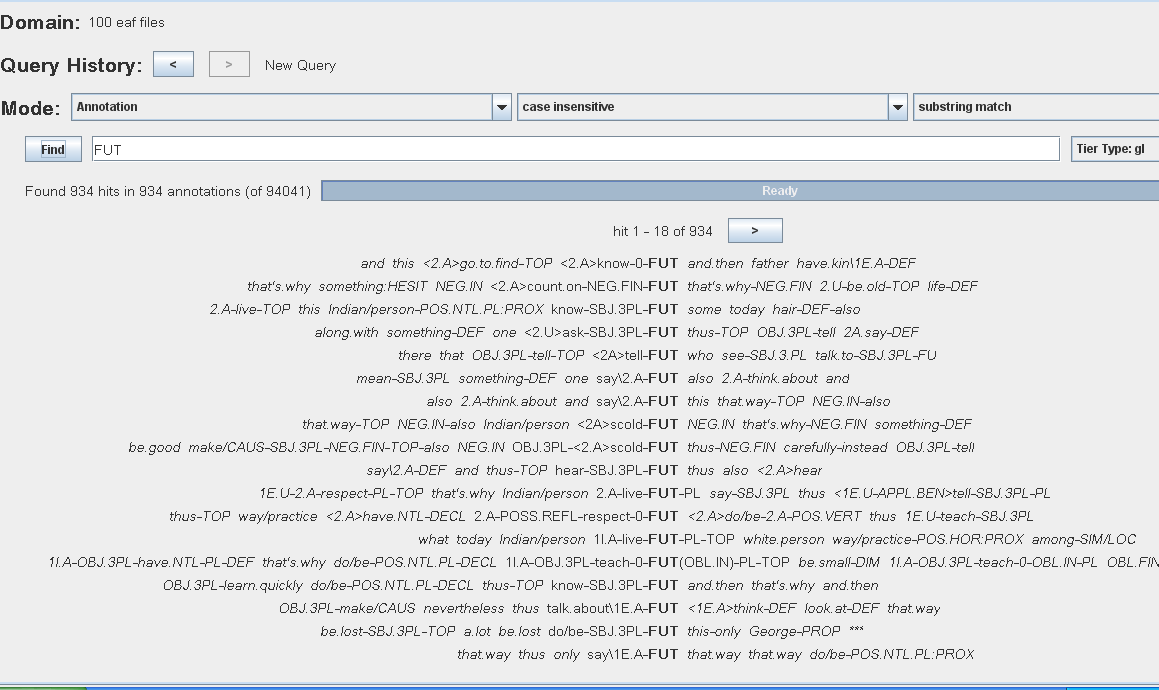
\includegraphics[width=\textwidth]{.\imgpath/BoudaSearchFUT.png}
\caption{Selection of hits of a search for the gloss \textsc{fut} (future tense marker) in the gl tier}
\label{bouda:fig:futuresearch}
\end{figure}


Another question would be: how to examine morphophonemic processes with corpus linguistic methods in DOBES corpora. Hoc{\A}k has heavy morphophonemic processes in the prefixes, i.e. the outcome of the combination of two prefixes often results in a very opaque form. See, for instance, \textit{h{\U}{\U}ro\v{g}oc} 'he was looking at me' which appears in example \ref{bouda:ex:HOR068}. The underlying form is: \textit{ho-{\II}-{\OO}-ro\v{g}oc} with a divided stem \textit{ho-ro\v{g}oc} 'look at' and the pronominal infixes 1\textsc{sg.ug}(me)-\textsc{3sg.a}(he). 
 
\ea\label{bouda:ex:HOR068}
ref HOR068
\glll 
tx Heg{\U} wogitekji        \textbf{h{\U}{\U}ro\v{g}oc}         \\
mo heg{\U} woogitek-xj{\II} \textbf{ho$<${\II}-\O-$>$ro\v{g}oc}   \\
gl that.way be.angry-\textsc{ints}   \textbf{$<$1\textsc{e.u}-\textsc{3sg.a}$>$look.at}        \\
\glll
tx wa'{\U}{\A}k\v{s}{\A}n{\A}, heg{\U} 'eeja n{\U}{\U}giw{\A}kj{\II}  \\  
mo wa'{\U}-'{\A}k-\v{s}{\A}n{\A} heg{\U} 'eeja n{\U}{\U}giw{\A}k-j{\II} \\
gl do/be(\textsc{sbj.3sg})-\textsc{pos.hor}-\textsc{decl} that.way there run-\textsc{ints}                    \\
\glll
tx kirikere haa. \\
mo kiri-kere haa \\
gl arrive.back.here-go.back.there make/\textsc{caus}{\textbackslash}1\textsc{e.a}\\

ft He was looking at me real mad and I left there running fast.\\
dt 25/Sep/2006\\
\z

What happens here is that the underlying pronominal affixes merge with the first part of the stem in quite unpredictable ways. The morphophonemic process can easily be examined by comparison of the gloss in the gl tier with the form in the text tx tier. In order to find out, whether this type of morphophonemic process happens regularly, one may search for the string \textit{h{\U}{\U}} in the text tx tier to get all instances of this process. Unfortunately, this search gives also words that are not inflected in this way such as \textit{h{\U}{\U}c} 'bear' and \textit{h{\U}{\U}k} 'chief'\textbf{\textit{.}} A solution would be to search across tiers, the form \textit{h{\U}{\U}} itself in the tx line, and the function 1\textsc{sg.ug}-\textsc{3sg.a} in the gl tier, in order to avoid to get all words that begin with \textit{h{\U}{\U}-}. 

\subsection{Beyond the word level}
\label{bouda:sec:beyondthewordlevel}

Structural units beyond the word level of complexity comprise grammatical categories that are expressed analytically, the internal structure of different phrase types such as the NP, the VP, the PP and so on, the constituent structure of the clause and the structure of complex clauses. The descriptive task of a structural grammar is to describe the internal structure and the distribution of these syntactic categories and constructions. For instance, in order to describe the NP as a syntactic category one has to find out the kinds of elements that may be combined in a NP and their possible order(s) within this constituent type. The problem for the corpus linguistic methods is that DOBES corpora do not have a syntactic annotation. Neither parts of speech nor phrases such as NPs etc. are annotated. Therefore, the descriptive linguist is forced to formulate indirect search routines in order to identify the intended phrase type, e.g. a NP. For instance, in Hoc{\A}k, most NPs end with a determiner on the right edge. Searching for these determiners (e.g. definite and indefinite articles, demonstrative pronouns) could be a way to find NPs in the text corpus. However, many subordinate clauses have a definite article on the right edge too, so they have to be filtered out by a second procedure. Another problem would arise that there are also NPs that have no determiners in this slot. Another possibility would be to search for nouns assuming that they always occur in NPs. This is not possible, since parts of speech are not annotated. In addition, there are NPs without nouns as heads. 

So, it can be concluded that the lack of a syntactic annotation hinders the corpus linguistic treatment of DOBES corpora quite a bit. It would be desirable to have a tool for the automatic or semi-automatic syntactic annotation of DOBES corpora to make them apt for the searches the descriptive linguist needs to analyze the syntax of the target language. This holds for the phrase level, the clause level and the sentence level of syntagmatic complexity.

Another question are grammatical categories that are expressed analytically. In principle, there is the possibility to search for one element of such a construction and then to compare the hits which contain the second element of such a construction with the ones in which this element does not occur. The other possibility is to look for the whole construction, i.e. a combination of two elements that belong to the construction. In the search string one has to specify the two elements by strings of characters and the number of elements that may interrupt this construction by variables (with certain regular expressions). For instance, in Hoc{\A}k, the modal meaning 'must not' is expressed by means of a combination of the future suffix \textit{-- kje} and a separate word \textit{heesg\'e} following the verb. Both elements occur independently with a specific meaning, but in combination they have the meaning 'must not' which cannot composed out of the elements. In the Hoc{\A}k corpus, this construction has already been identified and was glossed accordingly, cf. \xref{bouda:ex:ALV022}: 
 
\ea   \label{bouda:ex:ALV022}
ref ALV022
\glll 
tx Ciir\'a\v{s}ge hi\v{z}{\k{\'a}}  paag\'axwigi heg{\U} wa\v{z}{\k{\'a}}         \\    
mo cii-ra-\v{s}ge hi\v{z}{\A} paagax-wi-gi heg{\U} wa\v{z}{\A} \\ 
gl house-\textsc{def}-also one write(draw){\textbackslash}1\textsc{e.a}-\textsc{pl}-\textsc{top} that.way something  \\
\glll
tx hij{\A}h\k{\'{i}}n{\A} hi\v{z}\'{\A} paag\'axwigi m{\A}{\II}xet\'e cii          \\
mo  hij{\A}h{\II}-ra hi\v{z}{\A} paagax-wi-gi m{\A}{\II}xete cii                                          \\
gl different-\textsc{def} one write(draw){\textbackslash}1\textsc{e.a}-\textsc{pl}-\textsc{top} white.person house            \\
\glll
tx paag\'axikjawi  heesgera h{\A}{\A}k\'e heesge                                    \\           
mo \textbf{paagax-i-kje-wi} \textbf{heesge-ra} h{\A}{\A}ke heesge                     \\         
gl \textbf{write(draw){\textbackslash}1\textsc{e.a}-0-\textsc{obl}.\textsc{in}-\textsc{pl}} \textbf{\textsc{obl}.\textsc{fin}-\textsc{def}} \textsc{neg}.\textsc{in} that's.why\\ 
\glll
tx hawin{\II} 'eegi jaagu waac\'i          \\                                 
mo haa-wi-n{\II} 'eegi jaagu wa-ha-cii       \\                               
gl make/\textsc{caus}{\textbackslash}1\textsc{e.a}-\textsc{pl}-\textsc{neg}.\textsc{fin} and.then what \textsc{obj}.3\textsc{pl}-1\textsc{e.a}-live \\
\glll
tx han{\A}kwigi heesge paag\'axwigi      \\                                   
mo ha-n{\A}k-wi-gi heesge paagax-wi-gi     \\                                 
gl 1\textsc{e.a}-\textsc{pos}.\textsc{ntl}.\textsc{pl}-\textsc{pl}-\textsc{top} that's.why write(draw){\textbackslash}1\textsc{e.a}-\textsc{pl}-\textsc{top} \\
\glll
tx woogit\'ekire.\\
mo woogitek-ire \\
gl get.angry/mad-\textsc{sbj}.3\textsc{pl}\\
ft When we drew a house, \textbf{we were supposed to draw the white man's house}, if we drew what we were living in or something different they would get mad.\\
dt 23/Jul/2007\\
\z

However, if this is not the case, one has to formulate a complex search or to formulate subsequent searches in order to identify constructions like these. 

\section{Functional grammar -- the onomasiological approach}
% \label{bkm:Ref283033425}
\label{bouda:sec:functionalgrammar}

The goal of the onomasiological approach to grammar is to describe in a systematic way the linguistic means by which in the target language a certain general function can be expressed. This approach to grammar requires searching for semantic functions/ concepts and operations that are considered to be necessary more or less for each language. They are therefore considered universal. It is self-evident that there cannot be a complete list of such functions. Table \ref{bouda:tab:functionaldomains} presents a summary of the most important (probably universal) tasks a language has to be able to fulfill. 
 

\begin{table} 
\footnotesize
\begin{tabular}{p{2cm}p{3cm}p{3cm}p{3cm}}
\textbf{domain} &
\textbf{basic functions} &
\textbf{representative concepts and operations} &
\textbf{lexical expressions and grammatical constructions in English as cues for certain semantic concepts}\\\hline
apprehension \&

nomination &
an entity is grasped by categorizing and individuating it; it is named by a label or a descriptive expression &
categorization, types of concepts, empathy &
\textsc{num}-\textsc{n}

\textsc{n}-\textsc{sg}/\textsc{pl}\\\hline
concept modification &
a concept is enriched, or an object is identified &
attribution, apposition, relativization &
\textsc{adj-n}, \textsc{ptc-n}, \textsc{n-rel} constructions, \textsc{pro/prop}-appositions\\\hline
reference &
a representation is related to and delimited within the universe of discourse &
determination, deixis, reference tracking &
\textsc{dem-n}, 

\textsc{def-n}, \textsc{in}\textsc{def-n}, 

\textsc{sap-pro},

Non-\textsc{sap} 3\textsuperscript{rd} person pronouns \\\hline
possession &
the relation of an entity to another one is established or inheres in one of them &
possession in reference, possessive predication, external possessors &
genitive attribute (-\textit{s/ of})

verbs of possession (\textit{have, belong})

dative of possession (e.g. \textit{carry sth. for so.})\\\hline
spatial orientation &
an entity is localized in space statically or dynamically &
reference points, local relations, spatial and gestalt properties of objects &
spatial adverbs

\textsc{n}\tief{1} \textsc{prep-n}\tief{2} constructions with \textsc{n}\tief{1} as the Figure (object localized) and N\tief{2} as the Ground (region/ frame of reference)\\\hline
quantification &
the extent of the involvement of a set of entities in a predication is delimited &
quantification in reference and in predication; counting, ordering &
\textsc{n}-\textsc{sg}/\textsc{pl}

\textsc{num/quant-n}

numeral adverbials 

cardinal and ordinal numbers\\\hline
predication &
information is attributed to a referent &
existence, situation, characterization &
X is Y

X is a Y/ Xs are Ys

there is a X

X is \textsc{prep} \textsc{np}

X is \textsc{poss.pro} Y

and many more constructions of location and possession\\\hline
participation &
a situation is articulated into an immaterial center and a set of participants and circumstants related to it and to each other &
control \& affectedness, central vs. peripheral roles, alignment of fundamental relations &
Semantic types of verbs as cues for different event types, verb classes\\\hline

\end{tabular}
\end{table}

\begin{table}
\footnotesize
\begin{tabular}{p{2cm}p{3cm}p{3cm}p{3cm}}
\hline
temporal orientation &
a situation is designed with respect to its internal temporal structure and limits and temporally related to another situation &
situation types, aspectuality, temporal relations &
perfective vs. imperfective aspect (only indirectly in English, but see the progressive aspect)

verb classes (stative vs. dynamic; cf. test with progressive)

\textbf{tense }

\textbf{(past (V}\textbf{\textit{-ed}}\textbf{), }

\textbf{present perfect (}\textbf{\textit{have/has}}\textbf{ V}\textbf{\textit{-ed}}\textbf{), }

\textbf{present (}\textbf{\textit{{\OO}}}\textbf{/ }\textbf{\textit{-s}}\textbf{) , }

\textbf{future (}\textbf{\textit{will}} \textbf{\textit{V}}\textbf{))},

temporal adverbials (\textit{yesterday, tomorrow, last month, next Monday}, etc.)\\\hline

illocution,

modality,

evidentiality

 &
a proposition is rendered relative to speaker, hearer and reality &
speech acts, obligation, volition, possibility, toning, evidentiality &
question words, question marks, 

verb first position as indicator for imperative clause, exclamation mark

modals such as \textit{want, like, must, have to, should}, \textit{may, can}, etc.\\\hline
contrast &
a concept or proposition is assessed qualitatively by comparison with similar ones &
negation, comparison, gradation, intensification &
referent negation (\textsc{neg}-N), predicate negation (\textsc{neg} V)

\textbf{comparison }

\textbf{(positive, comparative, superlative of the \textsc{adj})}

\textsc{dim/aug}\\\hline
nexion &
a situation is expanded into a complex one, or several situations are linked together &
speech reproduction, complementation,

interpropositional relations &
coordinating and subordinating conjunctions (such as \textit{and, but, while, because} etc.) as cues for interpropositional relations, coordinate clauses and subordinate clauses\\\hline
communicative dynamism &
a proposition is articulated in foreground and background &
discourse structure, functional sentence perspective (topicalization, focusing, \textbf{emph}asis) &
there is a X that ...

It is X that ...

\end{tabular}
\normalsize
 \caption{Functional Domains and the formal cues in English \citep[based on][]{LehmannEtAl2004}.}
\label{bouda:tab:functionaldomains}
\end{table}

Table \ref{bouda:tab:functionaldomains} contains general functions such as reference, possession, and spatial orientation which are fulfilled by various formal means cross-linguistically, but also intra-linguistically. The latter means that even in an individual language there are different means by which these functions are expressed formally. However, these general functions are too abstract to be searchable in the corpus, since these general functions are not or only indirectly annotated in the glossing tier, or are not or only indirectly coded in the translation language English in the translation line. In order to be able to search these general lexical or grammatical meanings/ functions, one has to find lexical items or construction in the translation language -- in the Hoc{\A}k corpus, it is English - that express the intended meaning/ function or are at least cues for constructions that express the intended function. In the right hand column in Table \ref{bouda:tab:functionaldomains}, lexical expressions and grammatical construction in English are enumerated that may serve as search cues for certain semantic concepts and functions. How one can search certain linguistic phenomena that are cues for certain semantic concepts and functions will be illustrated in the subsequent sections Section\ \ref{bouda:sec:tense} and Section\ \ref{bouda:sec:comparison}. The possibility to search for semantic concepts and function utilizing the information in the translation tier is the major advantage a parallel corpus like the ones of the DOBES projects has over traditional monolingual corpora. 

\subsection{Time in Hoc{\A}k}\label{bouda:sec:tense}

In order to find out how tense is expressed in Hoc{\A}k, one has different possibilities to search in the English translation language. One may search for tensed verbs in English such as the past tense form of verbs or the future category expressed by a verb-auxiliary construction. In addition, one may search for temporal adverbials that indicate the time relation of the English clause assuming that in the corresponding Hoc{\A}k clause, there will be a similar time adverbial. 

For instance, if one searches the standard future construction in English, the will plus verb construction it suffices to search the string ``will'' in the translation tier. One gets 314 hits of ``will'' in the Hoc{\A}k corpus. The corresponding Hoc{\A}k clauses can then be looked at to see if there is a corresponding grammatical marker indicating future tense. In almost all cases, one can find one of the above mentioned allomorphs of the future morpheme \textit{--kje}. An additional possibility is to conduct a combined search across tiers like ``will'' in the ft tier and NOT \textsc{fut} in the gl tier, in order to find out, if the hits in English correspond always to the future marker (\textsc{fut}) in Hoc{\A}k. Interestingly, there are cases when we find a potential marker -\textit{n{\A}{\A}} in Hoc{\A}k corresponding to the \textit{will}{}-construction in English; cf. \xref{bouda:ex:WIC008}.
 
\newpage
\ea    \label{bouda:ex:WIC008}
ref WIC008
\glll 
tx Taawusiregi wiic{\A}t'{\II}{\II}ran{\A}{\A}n{\A},              \\
mo taawus-ire-gi wiic{\A}t'{\II}-ire-\textbf{n{\A}{\A}}-n{\A}       \\
gl be.dried-\textsc{sbj}.3\textsc{pl}-\textsc{top} be.noticeable-\textsc{sbj}.3\textsc{pl}-\textbf{pot}{}-\textsc{decl}     \\
\glll
tx haa\v{s}ak hiiran{\A}{\A}n{\A}. \\
mo haa\v{s}ak hii-ire-\textbf{n{\A}{\A}}-n{\A} \\
gl be.crusty(\textsc{obj}.3\textsc{sg}) make/\textsc{caus}-\textsc{sbj}.3\textsc{pl}-\textbf{pot}-\textsc{decl}\\

ft When they are dry, they \textbf{will} become tough, hard like a shell.\\
dt 07/Jun/2005
\z


The use of the potential marker in Hoc{\A}k in this context in \xref{bouda:ex:WIC008} makes perfectly sense, since the context is a conditional clause expressing a strong probability in the irrealis and not a future event. The English will construction is obviously not sensitive for this categorial distinction. 

Similar search procedures can be performed for the other tense categories. For instance, to search for V-\textit{ed}, one may search for the string \texttt{ed{\textbackslash}b} in the regular expression mode (in Elan) in the ft tier and get	 about 3000 hits. Looking through the tx and mo tier of the hits one can see that there is no past tense marker in Hoc{\A}k. 

\subsection{Comparison in Hoc{\A}k}\label{bouda:sec:comparison}

Another illustrative example for a fruitful application of the onomasiological search strategy would be comparison. Hoc{\A}k has no grammaticalized comparative and superlative. But, how can one find out, how these concepts that are tightly bound to adjectives are expressed in Hoc{\A}k. Again, one can look into the ft tier in order to find comparative or superlative forms which can be compared with the corresponding expressions in Hoc{\A}k. The cues for comparative to look for in English are the ending \textit{--er} and the marker of the standard of comparison \textit{than}; e.g., \textit{fast-er than his horse. }The \textit{--er} alone is not a good cue for the comparative, because on gets all words that end in \textit{--er} (n=1820 among them \textit{father, after} etc.) and these are mostly not comparatives. Hence, \textit{than} would be the better cue. Not surprisingly, there are only 7 instances in the whole corpus. It seems this is a category that is strongly avoided. The strategies to express comparison in Hoc{\A}k are lexical as can be seen for instance in  \xref{bouda:ex:bear}.

 

\ea\label{bouda:ex:bear}
\glll 
tx h{\U}{\U}cr\'a \v{s}{\U}{\U}kj\'{\A}kra hirak\'isan{\II}k h{\U}{\U}cr\'a 'ee wam{\A}\v{s}c\'{\A}{\A}n{\A} \\
mo h{\U}{\U}c-r\'a \v{s}{\U}{\U}kj\'{\A}k-ra \textbf{hirak\'isan{\II}k} h{\U}{\U}c-r\'a \textbf{'ee} wam{\A}\v{s}c\'{\A}-n{\A}\\
gl bear-\textsc{def} wolf-\textsc{def} \textbf{compared} bear-\textsc{def} \textbf{he.\textsc{\textbf{emph}}} strong-\textsc{decl}\\
ft 'The bear is strong\textbf{er} \textbf{than} the wolf'(lit. 'The bear \textbf{compared with the wolf}, the bear, \textbf{HE} is strong.') \\
\z


In tx h{\U}{\U}cr\'a \v{s}{\U}{\U}kj\'{\A}kra hirak\'isan{\II}k h{\U}{\U}cr\'a 'ee wam{\A}\v{s}c\'{\A}{\A}n{\A}, the asymmetry between the bear and the wolf with regard to the dimension strength is expressed by means of a clause that indicates that there is a comparison and by means of a subsequent clause that focuses the entity that has more of the dimension. This is not a grammaticalized construction, but a possibility speakers invent ad hoc in order to express the concept. There are many other different possibilities to express comparative.

A similar situation can be found in Hoc{\A}k with regard to the superlative. One may choose as cue in English the ending \textit{...est/b} for a search in the ft tier. Of course, there are words in English that end in ..\textit{.est} like \textit{west} or \textit{rest} that are not relevant. The result would be that a) the superlative occurs very rarely, and b) that it is not a grammaticalized construction. One possibility to express a concept like the superlative in Hoc{\A}k would be lexically such as in \ref{bouda:ex:superlative}.

% tx w{\A}ak hak{\II}n{\'{\k{u}}}pra waihakra 'ee here\'en{\A},.

\ea\label{bouda:ex:superlative}
\glll
tx w{\A}ak hak{\II}n{\k{\'u}}pra   waihakra                   'ee     \\
mo w{\A}k  ha-k{\II}n{\k{\'u}}p-ra \textbf{wa-{\OO}-hihak-ra} 'ee       \\
gl male \textbf{coll}-sibling-\textsc{def} \textbf{3\textsc{pl}.\textsc{obj}-\textsc{3sg.a}-on.top-\textsc{def}} he.EMPH     \\

\glll
tx here\'en{\A}, {Adam Little Bear Jr.}, raa{\v{s}}r\'a 'Aah\'u Ru'{\A}g\'a      \\
mo here\'e-n{\A}, {Adam Little Bear Jr.}, raa{\v{s}}-r\'a 'Aah\'u Ru'{\A}-g\'a \\
gl be-\textsc{decl} {Adam Little Bear Jr.}, name-\textsc{def} Wing Raising-\textbf{pn}                        \\
\glll
tx higa\'ireen{\A}\\
mo higa-\'iree-n{\A}\\
gl call-they-\textsc{decl}\\

ft 'My younger brother, Adam Little Bear Jr., whose name was Raising Wings, is \textbf{the youngest} in the family' (lit. translation: `Of the male siblings, HE (my younger brother) was \textbf{on top of them}, Adam Little Bear Jr. he was called Raising Wings.' \citep[cf.][v]{WhiteEagle1988})\\
\z

The meaning of the superlative is that an entity has - with regard to a certain class of the same or comparable entities - the highest value on a certain dimension. In tx w{\A}ak hak{\II}n{\k{\'u}}pra waihakra 'ee here\'en{\A},, it is expressed that Adam Little Bear is the youngest in the family, i.e. with respect to the dimension youngness, he is the one who has the highest value on this scale. What is astonishing here is that it is the property youngness that is the reference scale. This scale is invoked in the previous context of this text segment, where the speaker speaks of the younger brother using the special term for this in Hoc{\A}k. 

In the subsequent section, we want to review and evaluate the searching and concordancing functionality of Elan and Poio in order to arrive at list of requirements a software has to offer in order to support semasiological and onomasiological analysis of corpus data.

\section{Software-based search and analysis of corpus data}
% \label{bkm:Ref296514870}\label{bkm:Ref312671330}
\label{bouda:sec:softwarebasesearch}
In order to be able to evaluate software tools for linguistic analysis we use the same approach taken in \citet{Nordhoff2008} and define a set of values and maxims. Values in this sense define certain criteria to judge the quality of a software from a user's perspective. As Nordhoff states ``some of these values can be conflicting'', which means that different users prefer different solutions. Still, we consider most of the following values relevant for our purpose of comparing the two packages Elan and Poio (and others not mentioned here, of course) for search and analysis tasks in linguistics. The values are presented as a list of numbered maxims that will later be used to judge whether or not a software tool is better regarding a given value. So the maxims presuppose a certain point of view regarding the values. The reader might not follow all of our assumptions, but all the maxims are derived from the practical application of the ideas to develop a descriptive grammar based on corpus analysis presented in this paper. Our maxims are:

\begin{enumerate}
\item Search results should be presented as interlinear text.
\item The user should be able to find the source utterance in its context in the original file from the search result.
\item The user should be able to search on all existing tiers.
\item Relationships among search terms:
 \begin{enumerate}
 \item It should be possible to define relationships among search terms on one tier.
 \item It should be possible to define relationships among search terms on different tiers.
 \end{enumerate}
\item The user should be able to search within search results.
\item Search should be possible in a set of files, not only in one file. The more file formats supported, the better.
\item The user should be able to search for substrings in annotations and use regular expressions.
\item It is better when the user is confronted with fewer dialogs and windows during one search tasks.\footnote{ This is only an approximation of the quality of the graphical user interface design; a full review of the usability of each tool is left for future research.}
\item It should be possible to export searches and search results, in order to save and archive them for later reference.
\end{enumerate}

The following two sections first give an overview of both software packages, specifically of the search and analysis functionality implemented in the tools. Each section will conclude with a summary that contains a rating of the tool according to the maxims we outlined above.

\section{Review of Elan search and analysis functionality}

One of the widespread tools in language documentation nowadays is Elan, a transcription and annotation software developed by the Max-Planck-Institute in Nijmegen, Netherlands.\footnote{\url{http://www.lat-mpi.eu/tools/elan/}} As Elan was developed specifically for transcription and annotation of audio and video files in the beginning, search and analysis functionality was only added later to the software. This led to the current situation, where this functionality is distributed among several menu options within the user interface. Regarding the search types and approaches to corpus linguistic methods for descriptive purposes presented in the first part of this paper, Elan offers the following three features that fulfill some of the requirements the descriptive linguist is striving for:

\begin{itemize}
\item Export multiple files as: list of words/annotations
\item Search multiple eaf (files)
\item Structured search multiple eaf (files)
 \begin{itemize}
 \item Substring search
 \item Single layer search
 \item Multiple layer search
 \end{itemize}
\end{itemize}

The ``Structured search multiple eaf'' feature is by far the most complex and elaborated. It is in itself divided in three dialogs which are listed above. All of the features work on what is called a ``domain'' in Elan. A domain in this sense is a batch of files. The user can create a domain, give it a name, and then add Elan files to that domain. Later, within each search and analysis feature, users first select a pre-defined domain and then carry out their search and analysis on that domain. The user is able to do several types of analysis through all of the listed features. The following sections will each describe one of the features, and relate their functionality to the search types that were described in Section\ \ref{bouda:sec:typologyofsearches}.

\subsection{Export multiple files}

By the ``Export multiple files'' feature, the user can export all words or annotations of a batch of files to a simple text file. Figure \ref{bouda:fig:elanexport} shows the export dialog for word lists. The user selects the tiers from which to export and defines a token delimiter. The default option is to use the pre-defined delimiters, which tokenize by punctuation. Another option is the frequency count (``Count occurrences'' option in the dialog), which is added tab-separated to each entry in the exported text file. If the user chooses the frequency count each word in the export file is then accompanied with a number how often this word occurs in all of the domain files.

\begin{figure}
 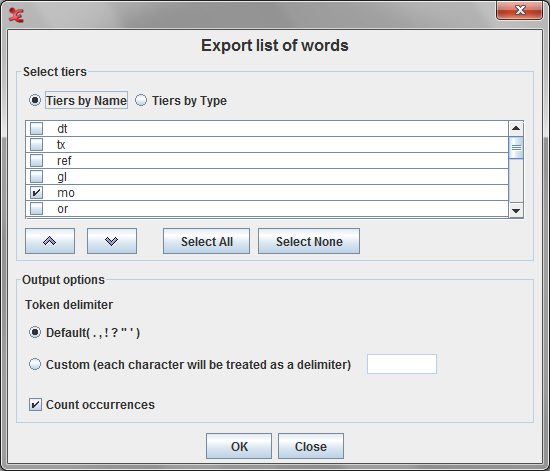
\includegraphics[width=\textwidth]{.\imgpath/Bouda-img9.png}
\caption{Word list export in Elan}
\label{bouda:fig:elanexport}
\end{figure}



Figure \ref{bouda:fig:extract} shows an extract of a sample export file of the Hoc{\A}k corpus. This method allows to some degree the identification of allomorphs of the word/lexeme as mentioned in Section\ \ref{bouda:sec:identificationoflexicaluntis}. The extract shows a list of words with a common prefix \textit{x{\U}n{\U}} `small, little'. Prefixed forms appear elsewhere in the list and have to be searched separately. Alternate stem vowels (long vs. short) will also lead to a separation of list entries with common lexical roots. The user is not able to trace back the entries to the corpus. Once the export is done, the user cannot simply jump to the position within the files where a list entry occurs. The export of the full interlinear context of words/annotations is not possible with Elan.

\begin{table}
\centering
\begin{tabular}{ll|ll}
Word form & frequency & Word form & frequency\\
\hline
x{\U}n{\U} & 1                     & x{\U}n{\U}-{\II}g-n{\A}{\A}gre &1  \\
x{\U}n{\U}-{\II}g & 1              & x{\U}n{\U}-{\II}g-ra & 1            \\
x{\U}n{\U}-{\II}g-i\v{z}{\A} & 1   & x{\U}n{\U}-{\II}k & 6               \\
x{\U}n{\U}-{\II}g-n{\A} & 1        & x{\U}n{\U}-{\II}k-ra &2             \\

\end{tabular}
\caption{Extract from the word list of the entire Hoc{\A}k corpus}
\label{bouda:fig:extract}
\end{table} 

\subsection{Search multiple eaf}

The second feature to be discussed here is the ``search multiple eaf'' option. This search functionality allows the user to search in the domain's eaf files for search terms. Search terms can be regular expressions or raw strings. The only other option in the search dialog is to switch on or off case sensitivity. Figure \ref{bouda:fig:multipleeaf} shows the search result dialog for the search term \textit{x{\U}n{\U}} `small, little'. In this case, the user is able to jump directly to the occurrence of the search term by double-clicking on any entry in the result list. In addition, the user is presented with the annotations before and after the search hit. This search is applied to all tiers in all files. It is not possible to restrict the tiers to search. The user can export the result list in a tab-separated format.

The search results are not displayed in full interlinear context, only a user-defined context on the same tier before and after the search term is shown.

\begin{figure}
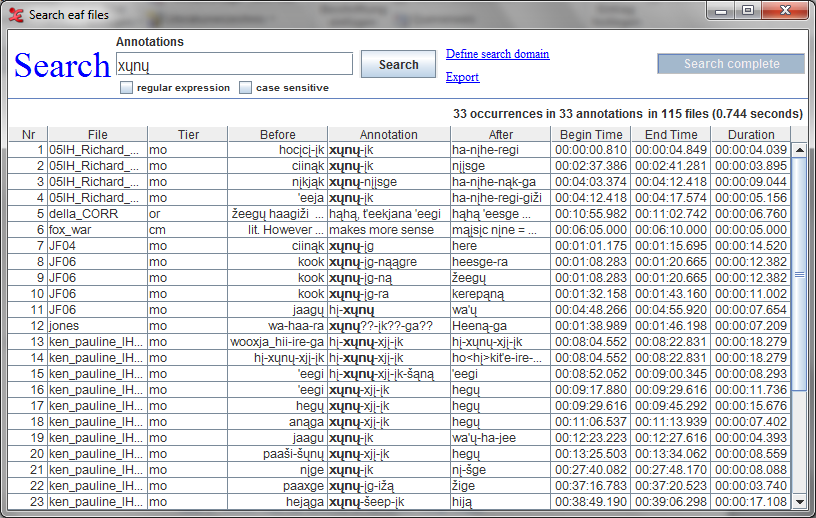
\includegraphics[width=\textwidth]{.\imgpath/Bouda-img10.png}
 \caption{Search multiple eaf in Elan}
\label{bouda:fig:multipleeaf}
\end{figure}



\subsection{Structured search multiple eaf}

Regarding the search typology presented in Section\ \ref{bouda:sec:typologyofsearches} above, the ``structured search'' is the most comprehensive facility for search and analysis in Elan. The ``structured search'' is in itself divided in three dialogs, hence search facilities: a simple substring search over all domain files, the single layer search and the multiple layer search. As only the latter two go beyond the ``search multiple eaf'' option already presented in the previous section, we will be only concerned with the search in layers here.

Figure \ref{bouda:fig:structuredsearch} shows both search dialogs. The left dialog presents a search for \textit{x{\U}n{\U}} in all tiers of the type mo. The ``multiple layers search'' is shown in the right dialog, with sample search for \textit{x{\U}n{\U}} in all tiers of type mo together with an occurrence of \textit{little} in tiers of type ft. In this example, the constraint between the tiers is set to ``No overlap''. The green boxes between search term boxes in the dialog allow the user to set different constraints within and between tiers. Constraints between tiers are concerned with different types of overlap, for example ``Left overlap'' or ``Within''. Constraints within a tier set the a maximum, minimum or exact distance of two search terms within the given tier, in terms of annotation counts or milliseconds within the media file.

 Both dialogs present the results in the lower parts of the dialog as concordances. The user can define the context size of the concordance. An alternative view is given by the ``frequency view'', in which all search hits are listed in a table with a count and a percentage. In both views the user can jump directly to the annotation in the eaf file by double-clicking on the element in the list view. The search results may also be exported to a tab-separated file with all timing and context information.

\begin{figure}
 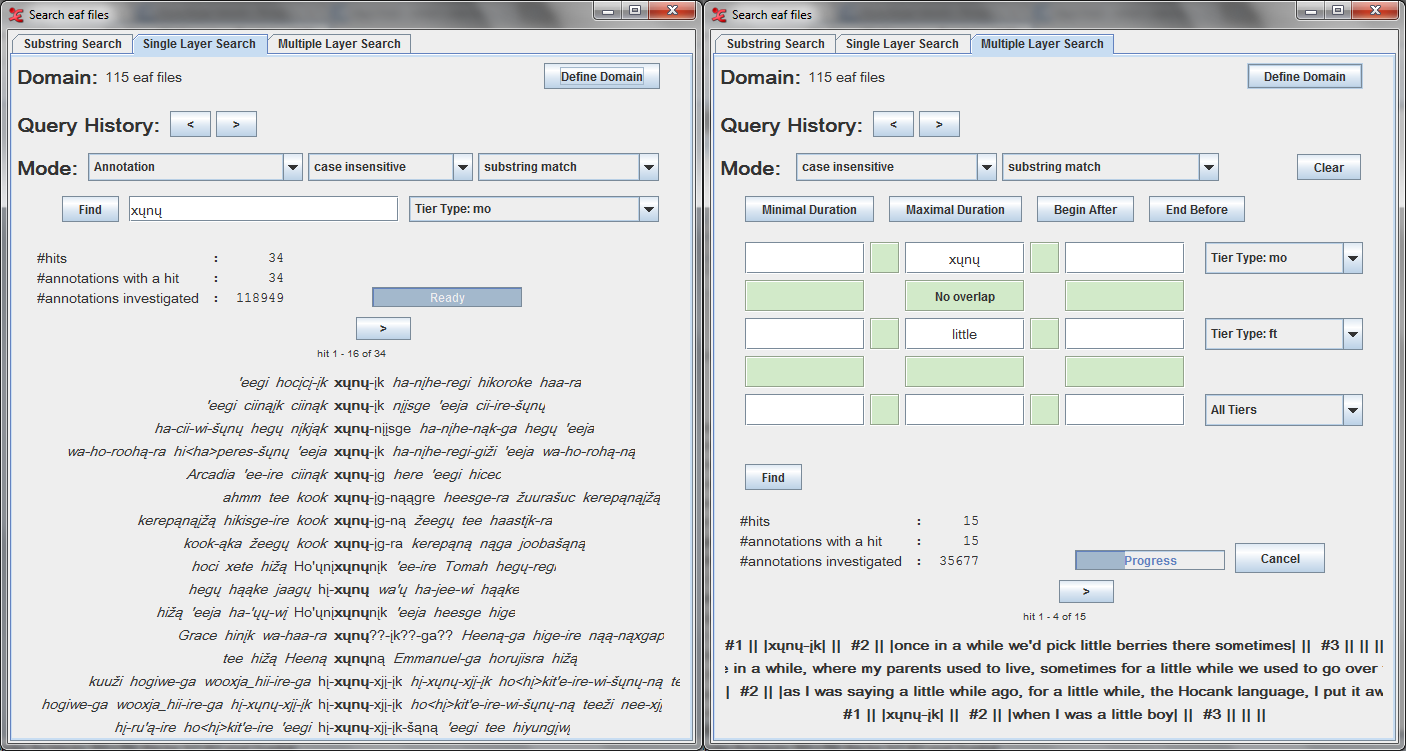
\includegraphics[width=\textwidth]{.\imgpath/Bouda-img11.png}
 \caption{Structured search in Elan}
\label{bouda:fig:structuredsearch}
\end{figure}

\subsection{Summary}
\label{bkm:Ref296713597}

Regarding the maxims in Section\ \ref{bouda:sec:softwarebasesearch}, the software Elan is rated as follows:

\begin{enumerate}
\item \textbf{Search results should be presented as interlinear text:}
It is not possible to view search results as interlinear text in Elan. Elan does not even display the annotation for all the tiers at the location where search strings occurs. Only the context within the tiers that was searched in is displayed. Elan does ignore this value completely.

\item \textbf{The user should be able to find the source utterance in its context in the original file from the search result.} 
The user is presented with a configurable context within the list of search results in the simple and complex searches. The user can click on each element in the list and Elan will open another window with the file of the search hit. The user than has to scroll left and right to see the context of the annotation and utterance within the file. We see problems in usability here, but in general Elan implements this feature.

\item \textbf{The user should be able to search on all existing tiers:}
Elan does allow searches on each tier without restrictions.
\item \textbf{Relationships among search terms:}

 \begin{enumerate}
 \item \textbf{It should be possible to define relationships among search terms on one tier;}
 \item \textbf{It should be possible to define relationships among search terms on different tiers:}

 Elan allows both types of connections between search terms. For some of our users in the project the connection names like ``overlap{\textquotedblright}, etc. were not very clear, so we think that usability could be improved. On the other hand the detailed connection types allow every thinkable search combination for the expert user.
 \end{enumerate}

\item \textbf{The user should be able to search within search results:}
Elan does not allow any further searches on the search result. 

\item \textbf{Search should be possible in a set of files, not only in one file. The more file formats supported, the better.}

Elan support searches in multiple files through its ``domain'' concept. But only one file format is supported directly, Elan's EAF format. The user may search in other file types by importing the files first and save them as EAF files.

\item \textbf{The user should be able to search for substrings in annotations and use regular expressions.}
Elan does fully support regular expressions.
\item \textbf{It is better when the user is confronted with fewer dialogs and windows during one search tasks.}\footnote{This 
 is only an approximation of the quality of the graphical user interface design; a full review is left for future research.}
Elan's search functionality is scattered among several menu options. So, the user has to open several menus and dialogs to try every possible search type. In the case of the export of word lists the user even has to open another application to apply the search. In our view Elan fails regarding this maxim.

\item \textbf{It should be possible to export searches and search results, in order to save and archive them for later reference.} It is possible to export the search results in Elan, but not the searches.
\end{enumerate}

In summary, Elan implements features for 6 of the 9 maxims. Maxims 1, 5 and 8 are violated completely, maxims 4, 6 and 9 only partly or only when we additionally take usability into account (in case of maxim 4). Elan's strength definitely is the structured search that allows advanced search strategies if the user learns about the connection types. Definitely missing is the interlinear view of search results, we also found major restrictions in getting context information from search results. Although the latter is possible, it is quite difficult for the user to get a quick overview of the search result and its context on all tiers at one glance.

\section{The Poio Analyzer for descriptive linguists}
\label{bouda:sec:poioanalyzer}
The development of the Poio Analyzer was started because we felt that Elan was not fulfilling all our needs. The software was planned as a tool for descriptive linguists working with data from language documentation projects from the beginning. Once the search typology emerged during the analysis of the Hoc{\A}k data, it became clear that Elan is not the right tool for a grammar writer to carry out the analysis. The development of the Poio Analyzer did not start from scratch though, as there was already a library for Toolbox and Elan file access (PyAnnotation\footnote{ \url{http://www.cidles.eu/ltll/poio-pyannotation}}) and a morpho-syntactic annotation editor (Poio ILE\footnote{\url{http://www.cidles.eu/ltll/poio-ile}}) available. The first provided a common API to the data files with access to the morpho-syntactic annotation, while the latter already contained a view to display utterances in an interlinear style. Both software packages were developed and used within the DOBES project ``Minderico --An endangered language in Portugal''.\footnote{\url{http://minderico.caorg.pt}} All software packages including Poio Analyzer are available for download on the Poio website\footnote{\url{http://www.cidles.eu/ltll/poio}} and are licensed under the GNU General Public License v3.0. Besides the source code there are installation packages for Windows available.

The following section will describe the user interface of Poio Analyzer, with a focus on the requirements that are missing in Elan and that Poio Analyzer implements. We will then give an outlook on future features that are currently work-in-progress before summarizing Poio's features and rating the software.

\subsection{The User Interface of Poio Analyzer}

Figure  \ref{bouda:fig:poioanalyzer} shows a screenshot of the Poio Analyzer. The main sections of the GUI are marked by numbered boxes. The example data in this screenshot show a search for the regular expression ``\^{}ra\$'' on the morpheme tier, the gloss ``\textsc{def}'' on the gloss tier and the word ``{\textbackslash}bthe{\textbackslash}b'' within the translation. The functionality of each part of the GUI surrounded by boxes is as follows:

\begin{enumerate}
\item Search tabs allow successive searches. Each ``New Search...'' tab filters on previous searches. Tabs allow changing intermediate searches by switching between the open tabs. Results are displayed for the current tab.
\item Input fields for search strings to search in each tier. Allows full-flavored regular expression through the updated Python regex module. E.g. character classes like {\textbackslash}w or {\textbackslash}b fully support Unicode; there is support for Unicode properties, blocks and scripts, etc.
\item Search options:

 \begin{enumerate}
 \item AND: matches, when all search strings of all tiers match.
 \item OR: matches, when one of the search strings matches.
 \item NOT: inverts the search result.
 \item ``contained matches'': this value alters the matches in the word, morpheme and gloss tier. If set, the search strings must match within the same word. Otherwise the search strings can match in the whole utterance. For example: if you search for ``ra'' in the morpheme tier, and for ``\textsc{def}'' in the gloss tier, the normal search will display all matches, where ``ra'' occurs in a morpheme plus all matches where ``\textsc{def}'' occurs in the gloss tier within one utterance. If ``contained matches'' is set the result will only contain matches where a word has ``ra'' in the morpheme tier and ``\textsc{def}'' in the gloss tier.
 \end{enumerate}

 \item Buttons for searches. Searches may be saved and restored; this will save all the search strings of all tabs.
 \item Here you can add or delete files from the corpus. The result view will be updated whenever the file list is changed.
 \item The result view. Matches are displayed in green color within utterances and translations. If there is a match on the word, morpheme or gloss tier the whole word and all its morphemes and glosses will be highlighted in green color. This allows the user to find the matches more easily. All utterances are always displayed with full interlinear annotations.
\end{enumerate}

\begin{figure}
 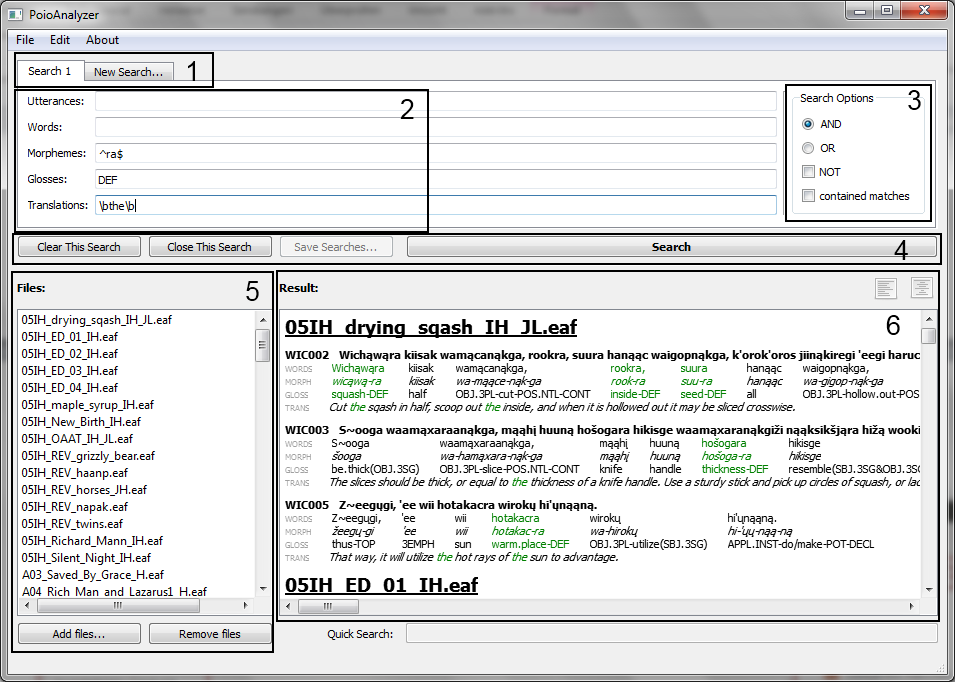
\includegraphics[width=\textwidth]{.\imgpath/Bouda-img12.png}
\caption{The GUI of Poio Analyzer}
\label{bouda:fig:poioanalyzer}
\end{figure}

The screenshot and its description demonstrate two of the most important requirements developed in Section\ \ref{bouda:sec:typologyofsearches}: search hits are presented in full interlinear context and the successive search functionality allows the user to conduct searches on previous search result sets. Both features already add value to the search functionality implemented in Elan and provide easier access to search results regarding the search typology developed in this paper. For example, morpho-phonemic processes as mentioned in Section\ \ref{bouda:sec:morphmebymorphemeglossing} can be analyzed by searching on the utterance and morpheme tier, with a logical AND operation and ``contained matches'' enabled. Another example is the search for word internal morphological structure as described in Section\ \ref{bouda:sec:wordinternalmorphologicalstructure}:  a search for the gloss ``\textsc{fut}'' with results in full interlinear context makes it easier to find out what kind of morphophonemic processes happen between the stems and the grammatical formative or between the combined forms of grammatical formatives. The biggest advantage of Poio Analyzer here is the view of results as interlinear version.

\subsection{Work in progress}

One of the features that were mentioned in Section\ \ref{bouda:sec:poioanalyzer} was the possibility to archive searches and result sets. This feature is currently not available in Poio Analyzer, but we plan to soon release an update that at least allows saving and restoring searches. Other functionality that we are currently working on is:

\begin{enumerate}
\item The possibility to search for set of words, morphemes, glosses, etc. This feature seems critical as it allows for example to search for word classes (e.g. part-of speech) which are not directly derivable from the annotations. In language documentation project there are often preliminary, sorted word lists available, that can be used for this kind of search. In the case of Hoc{\A}k a full dictionary is available, which we will use to search for word classes.

\item On top of this we want to make it possible to add part of speech annotation to the data. In the case of Hoc{\A}k there is part of speech information available in the dictionary. We are currently investigating the quality of part of speech tagging from this dictionary. Part of speech information would allow search for argument structures as described in Section\ \ref{bouda:sec:beyondthewordlevel}.

\item Add statistical evaluation of search result sets. This will be a simple count and percentage value for each tier first. Later, more advanced statistical methods may be added, depending on the needs of the users. The statistical view will also give access to list of words, morphemes and glosses in the result set. Those lists may then be exported and/or used for the ``set search'' described in 1.
\end{enumerate}

In addition to this we are always collecting ideas for improvement from our users. Depending on the complexity and necessity we will implement anything that seems useful to the descriptive linguist.

\subsection{Summary}

Regarding the maxims in Section\ \ref{bouda:sec:softwarebasesearch},the software Poio is rated as follows:

\begin{enumerate}
\item \textbf{Search results should be presented as interlinear text.}Poio does display all search results as interlinear text.
\item \textbf{The user should be able to find the source utterance in its context in the original file from the search result.}Poio does only view the utterance of the search hit. The context of the hit within the utterance is displayed completed, but utterances before and after the search hit are not presented to the user.
\item \textbf{The user should be able to search on all existing tiers.}Poio allows searches over all tiers that are relevant for interlinear texts. Additional tiers (that are not part of the hierarchy of a given utterance tier) are not supported yet.
\item \textbf{Relationships among search terms:}

 \begin{enumerate}
 \item \textbf{It should be possible to define relationships among search terms on one tier.}
 \item \textbf{It should be possible to define relationships among search terms on different tiers.}
 Poio does support both types of relationships, but not as elaborated as in Elan. For example it is not possible to restrict the search on a given tier with information about context size (''[search term 1] with a maximum distance from [search term 2]{\textquotedblright}).
 \end{enumerate}
\item \textbf{The user should be able to search within search results.}This is fully supported by Poio's successive search functionality.
\item \textbf{Search should be possible in a set of files, not only in one file. The more file formats supported, the better.}Poio supports Elan EAF, Toolbox TXT and Kura XML files. Files with different formats may be opened in parallel. The search is carried out over all open files.
\item \textbf{The user should be able to search for substrings in annotations and use regular expressions.}Regular expressions are fully supported by Poio.
\item \textbf{It is better when the user is confronted with fewer dialogs and windows during one search tasks.}\footnote{This 
 is only an approximation of the quality of the graphical user interface design; a full review is left for future research.
}

Poio follows this maxim, it only consists of one dialog.
\item \textbf{It should be possible to export searches and search results, in order to save and archive them for later reference.} Poio does currently not support this feature.
\end{enumerate}

In summary Poio implements features for at least 7 of the 9 maxims. Maxims 2 and 9 are not supported, implementation of features is only planned for future releases. In addition, maxim 3 and 4 are partly violated, as Poio does not support searches on all tiers if they are not part of the interlinear text convention. Combinations of search terms have certain restrictions, especially for searches on a single tier. If we take all the maxims into account Poio supports more of the ideas expressed by the values than Elan. It definitely has an advantage regarding usability, as it was developed as a special purpose tool for search and analysis. Elan, as a general purpose tool, has a lot of other features, like the possible to edit the files during analysis. The possibility to combine search terms in advanced ways is currently a standout feature of Elan.


\nocite{HartmannEtAl2009hocank}